\documentclass[]{afit-etd}
% \usepackage[square,sort&compress,numbers]{natbib} % Provides formatting for
                                                  % citations
\usepackage{textcomp} % Provides math symbols that can be used in text mode
\usepackage{amssymb}  % Provides additional AMS math symbols.  Note that
                      % amsmath is loaded as part of the afit-etd class
\usepackage{bm}       % Provides bold-faced math symbols
\usepackage{booktabs} % Provides improved table formatting
\usepackage{dcolumn}  % Provides table columns aligned at decimal points
\usepackage{multirow} % Provides table elements spanning multiple rows
% \usepackage{multicol}   % ??
\usepackage{graphicx} % Standard package to incorporate graphics
\usepackage[printonlyused]{acronym} % Provides a method for incorporating
                                    % acronyms and building an acronym list
\usepackage{subfigure} % Create subfigures
\usepackage{subfig}
\usepackage{calc}      % allows simple and easy calculations
\usepackage{wrapfig}   % wrapped text around figures - perhaps not appropriate
                       % in a thesis, but useful in general
% \usepackage[numbered]{mcode} % easily integrates matlab code
\usepackage{float} %H places the figure or tables in that exact location
\usepackage{amsthm}
\newtheorem*{definition}{Definition}
\usepackage{pdfpages}
\usepackage{subfigure} % Create subfigures
\usepackage{float} %H places the figure or tables in that exact location
\usepackage{multirow}
\usepackage{longtable}
\usepackage{tabu}
\usepackage{tikz}
% \usepackage{caption}
% \usepackage{subcaption}


%\usepackage{ifpdf} % \ifpdf ... \else ... fi structure
%\ifpdf 
%  \usepackage[pdftex, bookmarks, breaklinks,
%              plainpages=false,% Make page anchors using the formatted form of 
%                               % the page number. With this option, hyperref 
%                               % writes different anchors for pages 'ii' and
%                               % '2'. (If the option is set 'true' - the 
%                               % default - hyperref writes page anchors as the
%                               % arabic form of the absolute page number, 
%                               % rather than the formatted form.) [UK TeXfaq]
%              pdfpagelabels,   % Set PDF page labels; i.e., write the
%                               % value of \thepage to the PDF file so that
%                               % Acrobat Reader can display the page number as
%                               % (say) 'ii (4 of 40)' rather than simply '4 of
%                               % 40'. [UK TeXfaq]
%              colorlinks,      % use color instead of boxes for links
%              linkcolor=black, % color internal links black
%              urlcolor=black,  % color url's black
%              citecolor=black, % color links to references black
%              ]{hyperref} 
%\else  
%  \usepackage[hypertex]{hyperref}
%\fi


%% Required front matter definitions

\degree    {Doctor of Philosophy in Astronautical Engineering}
\graduation{March}{2015}
\designator{AFIT-ENY-15-M-??}

\title           {\MakeUppercase{Optimal Design of Dynamically Controlled Optical Systems}}
%\title{CHARACTERIZATION}

\author          {Timothy E. Coon} 
\rank            {Civilian}
\previousdegrees {BSME,MS} % Abbreviate any previous degrees

\committee{
  {Richard G. Cobb, PhD (Member) (Chairman)},
  {William P. Baker, PhD (Member)},
  {Michael R. Hawks, PhD ( Member)}
}

\department {Department of Aeronautics and Astronautics}
\school     {Graduate School of Engineering and Management}

 \dean       {M. U. Thomas} % only shows up for PhDs

\abstract{Chromotomographic imaging (CTI) offers advantages in remote sensing by resolving intensity distribution spatially, spectrally, and temporally. The \acf{CTEx} at the \acf{AFIT} explores the application of CTI as a space-based observer. Previous work in instrument development has revealed many of the intricacies of component fabrication and how they impact the resolving of image data. The proposed \ac{CTEx} instrument has as its chromatic dispersion element a \ac{DVP} that is made to rotate in order to achieve multiple projection angles. The inability to reconstruct a fast-transient scene has been largely attributed to the fabrication and alignment imperfections in the \ac{DVP} and so inspire improvement of the techniques for realizing a spinning \ac{DVP} optical element. The research herein presents an investigation into precise characterization of a \ac{DVP} and a proposed mechanical design of the \ac{DVP} hardware. The findings of this investigation provide the tools to specify fabrication tolerances for the \ac{DVP} and advance the research effort.

}

%% Optional definitions. 
%%Dedication has been commented out
\dedication{ \textit{to my grandfather \\ \hspace{20 mm} \\ ``Everything is an obvious extension of mechanical engineering." \\ \hspace{20 mm} \\  \hspace{6 cm} -GFG}}
\acknowledgments{I love my wife.
}
%% If you prefer to provide "acknowledgements" instead (note the added "e"
%% between the "g" and the "m") then add the "e" in the macro name so that
%% it reads "\acknowledgements".}

%% There is a predefined list of symbols that can be generated from symbols
%% marked in the text by "\addsymbol{Definition}{Symbol}".  If the symbols are
%% too wide for the table, the allotted width can be increased by including
%% an optional width in square brackets, as in  "\listofsymbols[.3in]".  
%% Similarly, a list of abbreviations is possible, corresponding to
%% "\addabbrev{Definition}{Symbol}".  Both of these lists will be ordered by 
%% number.

%% Additional "lists" can be added to the end of the front matter using the
%% \addlistof macro.  For example:
%\addlistof{Symbols}{Insert your list of symbols here or comment out this line.}
%% Note that the command "\input{symbols}" can be used if the symbol list is
%% contained in a separate file called "symbols.tex"}  In this example, the 
%% symbol list is assumed to be generated manually or using some other package

\addlistof{Acronyms}{\begin{singlespace}
\begin{acronym}
\setlength\itemsep{0pt}
\setlength\parskip{0pt}
\acro{2D}{two-dimensional}
\acro{3D}{three-dimensional}
\acro{AFIT}{Air Force Institute of Technology}
\acro{AVIRIS}{Airborne Visible/Infrared Imaging Spectrometer}
\acro{CAI}{Cloud and Aerosol Imager}
\acro{CAT}{Computed Axial Tomography}
\acro{CCD}{charge coupled device}
\acro{CMOS}{Complementary Metal-Oxide Semiconductor}
\acro{COTS}{commercial-off-the-shelf}
\acro{CRT}{cathode ray tube}
\acro{CTEx}{Chromotomography Experiment}
\acro{CT}{computed tomography}
\acro{CTI}{chromotomographic imaging}
\acro{DDE}{Dynamic Data Exchange}
\acro{DVP}{direct-vision prism}
\acro{EM}{electromagnetic}
\acro{EO}{electro-optic}
\acro{FBP}{filtered backprojection}
\acro{FFT}{Fast Fourier Transform}
\acro{FPA}{focal plane array}
\acro{FPN}{fixed-pattern noise}
\acro{FOV}{field-of-view}
\acro{FS}{Field Stop}
\acro{FTIR}{Fourier transform infrared spectroscopy}
\acro{FTS}{Fourier Transform Spectrometer}
\acro{FWHM}{full-width half-maximum}
\acro{GCTEx}{ground-based chromotomographic experiment}
\acro{GDT}[GD\&T]{geometric dimensioning and tolerancing}
\acro{HCI}{hyperspectral chromotomographic imager}
\acro{HSI}{hyperspectral imager}
\acro{IED}{Improvised Explosive Device}
\acro{IR}{infrared}
\acro{ISS}{International Space Station}
\acro{JPL}{Jet Propulsion Laboratory}
\acro{LMSE}{Laplacian Mean Square Error}
\acro{LSI}{linear-shift-invariant}
\acro{LWIR} {longwave infrared}
\acro{MSE}{Mean Square Error}
\acro{MTF}{Modulation Transfer Function}
\acro{MWIR} {midwave infrared}
\acro{NASA}{National Aeronautics and Space Administration}
\acro{NIR}{near infrared}
\acro{OLI}{Operational Land Imager}
\acro{POCS}{Projection Onto Convex Sets}
\acro{PSF}{point spread function}
\acro{PSNR}{peak signal-to-noise ratio}
\acro{PTF}{Phase Transfer Function}
\acro{OTF}{Optical Transfer Function}
\acro{QE}{quantum efficiency}
\acro{SAA}{Shift-and-Add}
\acro{SC}{Structural Content}
\acro{SNR}{signal-to-noise ratio}
\acro{STF}{System Transfer Function}
\acro{SVD}{Singular Value Decomposition}
\acro{SWIR} {shortwave infrared}
\acro{TRL}{technology readiness level}
\acro{USAF}{United States Air Force}
\acro{USGS}{United States Geological Survey}
\acro{VIS}{visible}
\end{acronym}
\end{singlespace}
}
%% Use "\begin{singlespace}
\begin{acronym}
\setlength\itemsep{0pt}
\setlength\parskip{0pt}
\acro{2D}{two-dimensional}
\acro{3D}{three-dimensional}
\acro{AFIT}{Air Force Institute of Technology}
\acro{AVIRIS}{Airborne Visible/Infrared Imaging Spectrometer}
\acro{CAI}{Cloud and Aerosol Imager}
\acro{CAT}{Computed Axial Tomography}
\acro{CCD}{charge coupled device}
\acro{CMOS}{Complementary Metal-Oxide Semiconductor}
\acro{COTS}{commercial-off-the-shelf}
\acro{CRT}{cathode ray tube}
\acro{CTEx}{Chromotomography Experiment}
\acro{CT}{computed tomography}
\acro{CTI}{chromotomographic imaging}
\acro{DDE}{Dynamic Data Exchange}
\acro{DVP}{direct-vision prism}
\acro{EM}{electromagnetic}
\acro{EO}{electro-optic}
\acro{FBP}{filtered backprojection}
\acro{FFT}{Fast Fourier Transform}
\acro{FPA}{focal plane array}
\acro{FPN}{fixed-pattern noise}
\acro{FOV}{field-of-view}
\acro{FS}{Field Stop}
\acro{FTIR}{Fourier transform infrared spectroscopy}
\acro{FTS}{Fourier Transform Spectrometer}
\acro{FWHM}{full-width half-maximum}
\acro{GCTEx}{ground-based chromotomographic experiment}
\acro{GDT}[GD\&T]{geometric dimensioning and tolerancing}
\acro{HCI}{hyperspectral chromotomographic imager}
\acro{HSI}{hyperspectral imager}
\acro{IED}{Improvised Explosive Device}
\acro{IR}{infrared}
\acro{ISS}{International Space Station}
\acro{JPL}{Jet Propulsion Laboratory}
\acro{LMSE}{Laplacian Mean Square Error}
\acro{LSI}{linear-shift-invariant}
\acro{LWIR} {longwave infrared}
\acro{MSE}{Mean Square Error}
\acro{MTF}{Modulation Transfer Function}
\acro{MWIR} {midwave infrared}
\acro{NASA}{National Aeronautics and Space Administration}
\acro{NIR}{near infrared}
\acro{OLI}{Operational Land Imager}
\acro{POCS}{Projection Onto Convex Sets}
\acro{PSF}{point spread function}
\acro{PSNR}{peak signal-to-noise ratio}
\acro{PTF}{Phase Transfer Function}
\acro{OTF}{Optical Transfer Function}
\acro{QE}{quantum efficiency}
\acro{SAA}{Shift-and-Add}
\acro{SC}{Structural Content}
\acro{SNR}{signal-to-noise ratio}
\acro{STF}{System Transfer Function}
\acro{SVD}{Singular Value Decomposition}
\acro{SWIR} {shortwave infrared}
\acro{TRL}{technology readiness level}
\acro{USAF}{United States Air Force}
\acro{USGS}{United States Geological Survey}
\acro{VIS}{visible}
\end{acronym}
\end{singlespace}
" if the acronym list is in a separate file called
%% "acronyms.tex".  Note that the formatting generated by the acronym package
%% can be forced into singlespaced text by inserting "\setlength\itemsep{0pt}
%% \setlength\parskip{0pt}" into the "acronym" environment.} 

%% The default disclaimer and copyright statement is included by default.  An
%% alternate disclaimer for foreign students or others can be defined here. 
% \govtdisclaimer{Alternate Disclaimer.//See the Style Guide for more information}    

%% The default distribution is "APPROVED FOR PUBLIC RELEASE; DISTRIBUTION 
%% UNLIMITED". If a limited distribution is required, it should be entered here
%\distribution{Distribution Statement C.//See the Style Guide for more information}

% \notables  % Prevent a list of tables from being created if not needed
% \nofigures % Prevent a list of figures from being created if not needed

%% Defining the following dates will cause the signature pages to be marked
%% with ``//signed//'' and the date. This avoids having to scan the signature
%% page into the final document.  
% \signedDate{21 March 2011}
% \deanSignedDate{21 March 2011} % Only for PhD dissertations

% command for inline comments
\newcommand{\comment}[1]{}

%command for multiline cells in a table
\newcommand{\specialcell}[2][c]{%
  \begin{tabular}[#1]{@{}c@{}}#2\end{tabular}}

\begin{document}

\makePrefatoryPages % Don't remove this - it generates the prefatory pages

\chapter{Introduction}
\label{ch:intro}

This thesis presents a mechanical engineering perspective on the investigation into the fabrication and alignment of a \acf{DVP} which is a component of the \acf{AFIT} \acf{CTEx}. The work herein investigates mechanical limitations in fabricating and aligning a \ac{DVP} assembly by utilizing optical diagnostic tools to drive systematic mechanical design. \ac{CTEx} is a long-running \ac{AFIT} research effort to promote space-based \acf{CTI} technology utilizing a rotating prism as the dispersive element in the optical system~\cite{Lemaster,Dearinger, Gustke, Gould}~\cite{ODell, ODellSPIE, Niederhauser}.

%This work was intended as an open-ended investigation and only the pertinent theory and observations as they pertain to the advancement of the CTEx project are detailed herein.

%%%%%%%%%%%%%%%%%%%%%%%%%%%%%%%%%%%%%%%%%%%%%%%%%%%%%%%%%%%%%%%%%%%%%%%%%%%%%%%%%%
\section{Motivation}
\label{sec:motivation}

 \ac{CTEx} is motivated by the spectroscopic capabilities of spinning-prism \ac{CTI} technology above the industry-leading imaging Fourier transform spectroscopy (imaging FTIR) approaches. The most significant advantages are presented in~\cite{Bostick08} by Bostick and Perram whose claim is that ``chromotomography offers several advantages over FTIR approaches, including: (1) simple design with less sensitivity to vibration, (2) easy integration with standard imaging sensors, and (3) the use of event phenomenology in the CT transform for increased temporal response"~\cite[p. 519]{Bostick08}. \ac{CTEx} achieves \ac{CTI} by utilizing a rotating \ac{DVP} dispersive element. An alternative approach to achieving \ac{CTI} is to use a non-rotating dispersive element and large optical detector arrays~\cite{Descour}. While each method of achieving \ac{CTI} offer advantages, the objective of \ac{CTEx} includes a spectral resolution of transient events that is not obtained by non-rotating designs. Further detail on the advantages of \ac{CTI} is presented in Section~\ref{sec:HSIres}.

Previous \ac{CTI} experiments conducted at \ac{AFIT} used prisms characterized by direct angle observations implemented to detail a wavelength-dependent dispersion profile. However, with the completion and operation of recent \ac{CTI} instruments by \ac{AFIT}, the limitations imposed on \ac{CTI} efficacy by the misalignment of the optical system were highlighted~\cite{Sue} \cite{Bostick}. The inability to reconstruct a fast-transient scene has been largely attributed to the fabrication and alignment imperfections in the \ac{DVP} and so inspire improvement of the techniques for realizing a spinning \ac{DVP} optical element \cite{HawksATF}. As is demonstrated by Bostick~\cite{Bostick}, the fabrication and installation alignment of the \ac{DVP} assembly has significant impact on the spatial and spectral information that can be obtained by the \ac{CTI} system. With new understanding as a result of \ac{AFIT} research efforts gone before, the need is established for a thorough investigation set on achieving an understanding of the practical limitations in precision installation alignment and fabrication of a \ac{DVP}.

%%%%%%%%%%%%%%%%%%%%%%%%%%%%%%%%%%%%%%%%%%%%%%%%%%%%%%%%%%%%%%%%%%%%%%%%%%%%%%%%%%
\section{Hyperspectral Remote Sensing}
\label{sec:hyperspectralRemoteSensing}

The \ac{CTEx} instrument is a proposed space-based hyperspectral remote sensor. An introduction to hyperspectral remote sensing is offered here beginning with a description of remote sensing in general.

\subsection{Remote Sensing}
\begin{quote}
Remote sensing is the science of deriving information about an object from measurements made at a distance from the object, i.e., without actually coming into contact with it. The quantity most frequently measured in present-day remote sensing systems is the electromagnetic energy emanating from the objects of interest... (D. A. Landgebe, quoted in Swain and Davis, 1978, p. 1) \cite{Campbell}
\end{quote}

The electromagnetic (EM) energy spectrum, in general, is the broad range of electromagnetic radiation defined by the frequency at which the energy oscillates perpendicular to the path it dominantly traverses. A spectral band, or spectrum, refers to a specified range of frequencies (or wavelengths) at which electromagnetic waves exist. As the total electromagnetic spectrum is continuous, the approximate extent of these ranges is often defined by common physical boundaries. For example, the visible spectrum is defined by the approximate range of electromagnetic radiation that is detectable by the human eye \cite{Hecht}. The ranges are illustrated in Figure~\ref{fig:EMspectrum} and detailed in Table~\ref{tbl:EMspectrumTable}, however, the range of each spectrum is specified differently by various references as each range is intractable due to a lack of universally-recognizable constraints. Throughout this work, where the wavelength of energy is used to classify a spectrum, the assumed medium is a vacuum because, overall, the frequency of electromagnetic energy remains constant, but the wavelength changes relative to the medium in which it travels according to Equation~\eqref{eq:wavelength}~\cite{Hecht}.

\begin{figure}[htb]		% EMspectrum
\centering
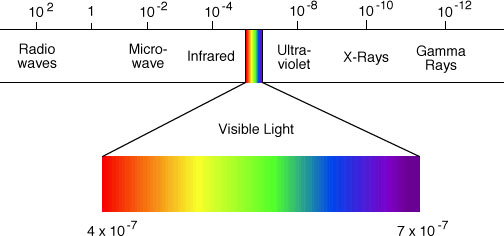
\includegraphics[width=0.75\textwidth]{images/chap1/EMspectrum}
\caption{Illustration of \acl{EM} spectrums with the visible spectrum highlighted~\cite{RedOrbit}.}
\label{fig:EMspectrum}
\end{figure}

\begin{table}[htb] 		% EMspectrumTable
\caption{Principle Divisions of the EM Spectrum} % title of Table 
\label{tbl:EMspectrumTable}
\centering % used for centering table 
\begin{tabular}{lr} % centered columns (2 columns)
\hline
Division & Limits \\  % inserts table heading 
\hline % inserts single horizontal line
Gamma Rays & less than 0.03 $nm$ \\
X-Rays & 0.03 - 300 $nm$\\
Ultraviolet Radiation & 0.30 - 0.38 \textmu m \\
Visible Light & 0.38 - 0.72 \textmu m \\
Infrared Radiation & 0.72 - 1000 \textmu m \\
 \hspace{.25cm} $\bullet$  Near infrared & 0.72 - 1.30 \textmu  m \\
 \hspace{.25cm} $\bullet$  Mid infrared & 1.30 - 3.00 \textmu  m \\
 \hspace{.25cm} $\bullet$  Far infrared & 7.00 - 1000 \textmu  m \\
Microwave Radiation & 1 - 300 $mm$ \\
Radio Waves & greater than 30 $cm$ \\
\end{tabular} 
\end{table}

\begin{table}		% eq:wavelength
\centering
\begin{equation}		% wavelength
\label{eq:wavelength}
\lambda = \frac{\nu}{f}
\end{equation}
\begin{tabular}{lll}
\singlespace
$\lambda$ & $\equiv$ & $\textit{wavelength in a medium}$ \\
$\nu$ & $\equiv$ & $\textit{speed of EM wave in a given medium}$ \\
$f$ & $\equiv$ & $\textit{frequency of the EM wave}$ \\
\end{tabular}
\end{table}

\subsection{Spectroscopy}
Spectroscopy is the study of electromagnetic waves separated by energy level, i.e. wavelength~\cite{Kulesa}. Spectroscopy enables the identification of chemical elements, in many cases, by direct, passive observation of electromagnetic waves as certain elements emit energy at sharply-defined wavelengths when chemical reactions occur or reflect only some wavelengths. Figure~\ref{fig:HgLampSpectrum} displays the amplitude of the energy released across the visible spectrum by current conducting through a mercury vapor lamp~\cite{Roberts}. The response profile is unique and, therefore, valuable, as there is no other event that emits energy with the exact same spectral profile. As such, this general event of current conducting through mercury vapor is positively identified by observation of its distinct emission. The unique wavelength profiles of emission or reflection for a material or event are known as spectral signatures~\cite{SpectralSignatures}.

\begin{figure}[htb]		% HgLampSpectrum
\centering
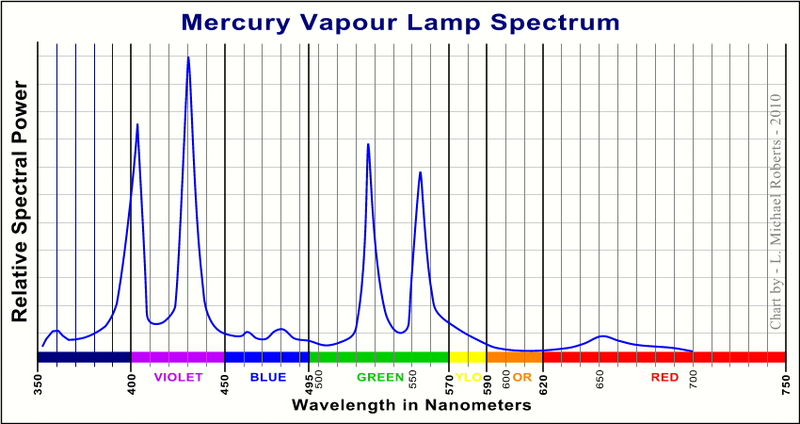
\includegraphics[width=.9\textwidth,trim=.1cm .1cm 2cm 1cm,clip]{images/chap1/HgLampSpectrum}
\caption{Spectral Signature of a mercury vapor lamp. The specific profile of power vs. wavelength shown is unique to the mercury vapor lamp~\cite{Roberts}.}
\label{fig:HgLampSpectrum}
\end{figure}

\subsection{Hyperspectral Remote Sensing}
\label{sec:HSI}
Hyperspectral remote sensing refers to the use of spectroscopy for observation of electromagnetic radiation within a uniquely-prescribed spectral band. To be considered hyperspectral, the energy observed must radiate at 0.4 to 14 \textmu m wavelength (20 to 750 THz frequency)~\cite{Sue} which encompasses the entire visible spectrum as well as parts of the \ac{SWIR} and the ultraviolet spectrums. The propensity for earth-imaging spectrometers to observe in the hyperspectral bandwidth is attributed to the assiduous tendency of the Sun to illuminate the Earth. The significance of solar illumination is evident in Figure~\ref{fig:RemoteSensing} showing that the energy detected by an Earth-observing satellite is largely the Sun's reflected radiation. Figure~\ref{fig:SolarEmissionSpectrum} shows that the greatest magnitude of received solar radiation occurs inside the hyperspectral bandwidth. Because the earth is illuminated by the hyperspectral bandwidth, it also reflects significantly in the hyperspectral bandwidth supplying ample signal for remote-sensing instruments. Furthermore, hyperspectral imagers are distinguished from other imagers by boasting a significantly higher spectral resolution than do other earth-sensing spectrometers~\cite{Shippert}. Greater spectral resolution is defined by more numerous and more narrow bandwidths within the designated spectrum. Higher spectral resolution allows for more precise definition of the signal received. Figure~\ref{fig:Reflectance} illustrates the spectral information inherent to an observed scene.

% note: "radiation" is the process of waves travelling, "emission" is the process of generating those radiation waves

\begin{figure}[htb]		% RemoteSensing
\centering
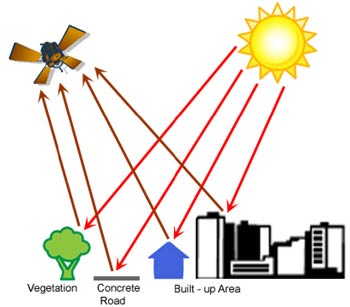
\includegraphics[width=0.5\textwidth]{images/chap1/RemoteSensing}
\caption{The radiation detected by an Earth-observing satellite has a significant contribution from solar emission~\cite{RemoteSensing}.}.
\label{fig:RemoteSensing}
\end{figure}

\begin{figure}[htb]		% SolarEmissionSpectrum
\centering
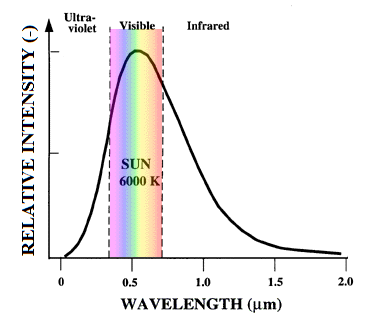
\includegraphics[width=0.5\textwidth]{images/chap1/solaremissionspectrum}
\caption{The solar emission spectrum indicates that most of the solar radiation reaching earth is in the low-end of the hyperspectral region of 0.4 to 14 \textmu m~\cite{JunkScience}.}
\label{fig:SolarEmissionSpectrum}
\end{figure}

% From a sampling-theory perspective, assuming equally-spaced, adjacent bandwidths, the spectral resolution or, the bandwidth of each spectral slice, defines the Nyquist frequency for the sampled signal. If the detected signal intensity vs. frequency curve contains frequency contribution above the Nyquist frequency, then the signal representation is degraded due to aliasing. With this relationship, the required bandwidth is be chosen based on an estimated signal profile of the desired targets. This is especially important as the transmittance of the atmosphere varies with the wavelength. This concept is illustrated in figure~\ref{fig:Reflectance}.

\begin{figure}[htb]		% Reflectance
\centering
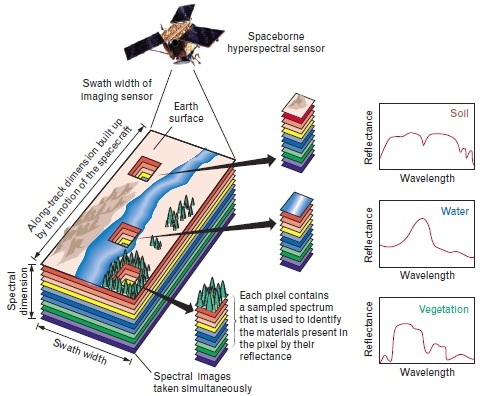
\includegraphics[width=1\textwidth]{images/chap1/ReflectanceSpectrum}
\caption{Spectral signature inherent to the scene at various points sensed by a hyperspectral imager~\cite{Shaw}.}
\label{fig:Reflectance}
\end{figure}

\subsection{The Hypercube}
A hyperspectral imager extracts from a signal the intensity of numerous finite spectral bandwidths at discrete points within the field of view. To visualize these datasets, the hypercube is often presented as shown in Figure~\ref{fig:hypercube}, which is ground image data collected by the \ac{AVIRIS}. Each horizontal slice through the XY-plane of the hypercube displays the intensity of a particular bandwidth as it varies with location in the two-dimensional \ac{FOV}. The ideal hypercube presents a two-dimensional spatial distribution of signal intensity at each infinitesimal wavelength along the Z-direction, or a continuous variation in the spectrum.

\begin{figure}[htb]		% hypercube
\centering
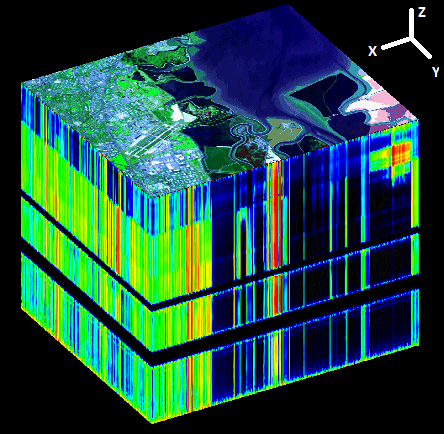
\includegraphics[width=0.75\textwidth]{images/chap1/avcubebig}
\caption{Hypercube taken from AVIRIS platform over Moffet Field, CA. Each cross section parallel to the XY-plane is the two-dimensional spatially-resolved emission intensity over the field of view at an infinitesimal spectral band. The wavelength of the energy varies continuously in the Z-direction~\cite{AVIRIS}}.
\label{fig:hypercube}
\end{figure}

\subsection{Hyperspectral Imager Temporal Resolution}
\label{sec:HSIres}
The performance measure of temporal resolution is not often discussed in relation to spectroscopy. However, it is an important aspect of hyperspectral imaging as many interesting targets evolve quickly both spectrally and spatially. To illustrate the relationship between spatial, spectral, and temporal resolution, examples are mapped onto a resolution triangle in Figure~\ref{fig:trifecta}. A hypercube is shown on the left and represents a spectrally- and spatially-resolved, two-dimensional static scene with low temporal resolution as the whole image is not associated with any one instant in time. An explosion is shown on the right and represents a spatially- and temporally-resolved event with no spectral-resolution beyond the color bands of the detector array. A chart of spectral change over time at the bottom is resolved for a finite area and offers no spatial resolution over the area. Because most imagers naturally exclude one element of the resolution triangle, some information is inherently lost. For hyperspectral imagers, the temporal aspect is most often traded for the information in the spatially- and spectrally-resolved hypercube. A closer look at hyperspectral imager instrumentation operation reveals the natural temporal exclusion.

\begin{figure}[htb]		% trifecta
\centering
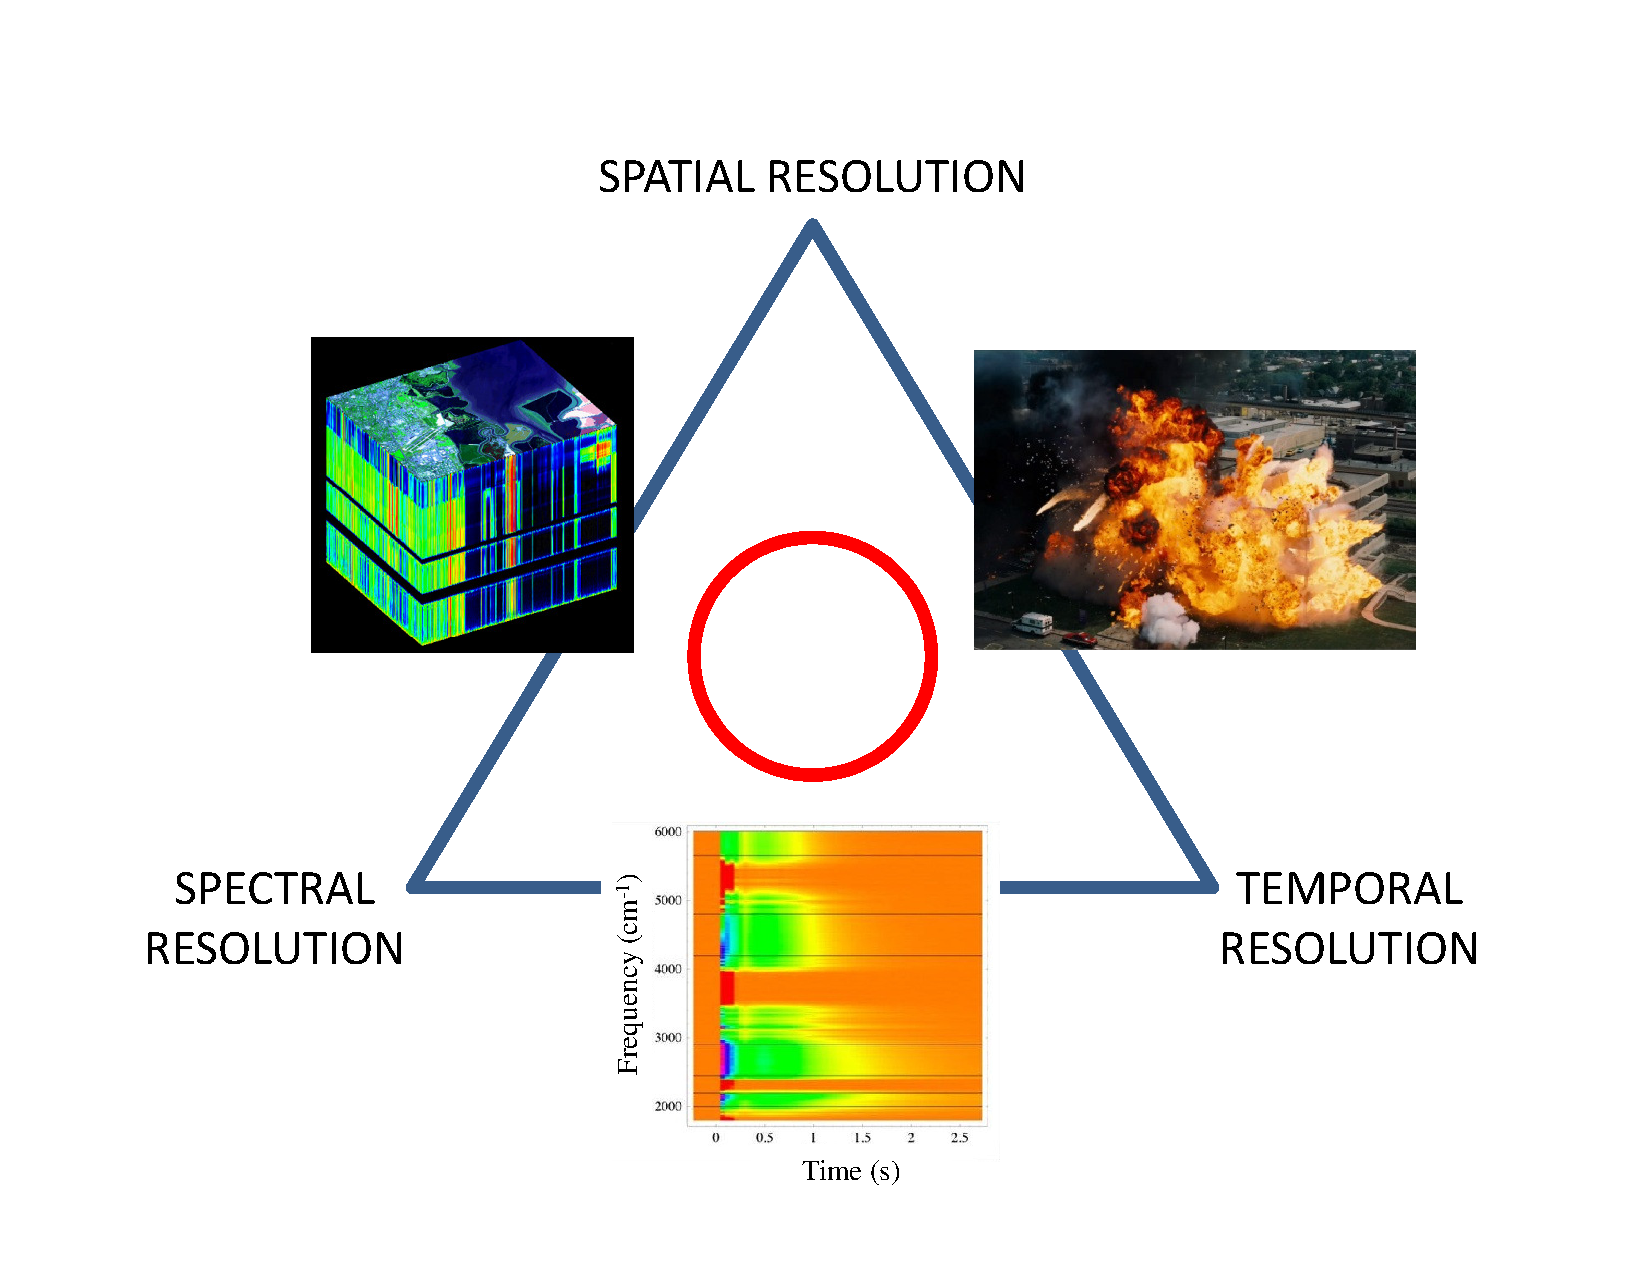
\includegraphics[width=1\textwidth,page=1]{images/chap1/MyGraphics_Ch1}
\caption{The resolution triangle illustrates the natural trades in image system resolution. Although not limited by general theory, realized imaging systems tend to achieve high resolution in only one or two of the three resolution types. CTI technology transcends this limitation~\cite{Niederhauser,DarkKnight}}.
\label{fig:trifecta}
\end{figure}

As discussed in Section~\ref{sec:hyperspectralImagers}, there have been and currently exist a number of space-based, earth-observing hyperspectral imagers. These imagers, by definition, generate highly-resolved intensity distributions as a function of spatial and spectral dimensions visualized by the hypercube of Figure~\ref{fig:hypercube}. The limitation of these and most spectrometers is that the time to collect the data to generate a spatially- and spectrally-resolved hypercube for a large \ac{FOV} is long enough that rapidly-changing events are not resolved temporally. Consider an imager such as EO-1 Satellite's Hyperion Imaging Spectrometer. This instrument operates as a push-broom spectrometer able to spectrally resolve a one-dimensional landscape as shown in Figure~\ref{fig:pushbroomOperation}. Because Hyperion and other push-broom spectrometers must resolve only individual thin slices of the \ac{FOV} at one time, the hypercube for the entire \ac{FOV} takes considerable time to integrate. If an explosion occurred within some segment of a two-dimensional area, Hyperion would either miss the event or only collect incongruous spectral information along one spatial line. 

 The solution to this temporal lapse is \ac{CTI}. The rapidly-rotating dispersion element projects the spectral information onto a spatial dimension and records, in multiple images, resolved spectral and spatial information for the hypercube many times per second. With implementation of \ac{CTI}, a space-based observer has the ability to survey a large ground swath area continuously and resolve spatial and spectral changes with time at any point within the \ac{FOV}. Thus, \ac{CTI} reaches all three corners of the resolution triangle in Figure~\ref{fig:trifecta}.
 
 \begin{figure}[htb]		% pushbroomOperation
\centering
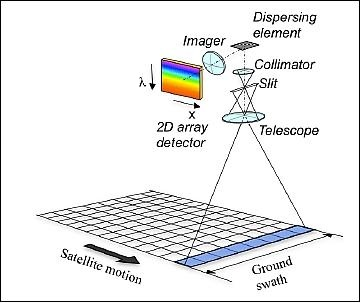
\includegraphics[width=0.5\textwidth,trim=0.25cm 0.25cm 0.25cm 0.25cm,clip]{images/chap1/pushbroomOperation}
\caption{A push-broom spectrometer resolves one narrow strip within the field of view at each integration~\cite{AVIRIS}}.
\label{fig:pushbroomOperation}
\end{figure}

\subsection{CTI Disadvantages}
Though \ac{CTI} offers resolution capabilities not achieved by other technologies, the advantages are not easily attained. As evidenced by the hard-earned advancement of the technology, \ac{CTI} hardware and theory is wrought with many intricacies and is highly-sensitive to numerous subtleties in instrument design and image processing. Pertinent to the research presented herein, it is shown that small imperfections and uncertainties in \ac{DVP} fabrication result in highly degraded results. \ac{CTI} relies on the alignment of optical components to sub-wavelength precision. While this is obviously accomplished in countless optical systems, few must maintain these tolerances while combating the disturbances of the \ac{DVP} rotating at high speed.

%%%%%%%%%%%%%%%%%%%%%%%%%%%%%%%%%%%%%%%%%%%%%%%%%%%%%%%%%%%%%%%%%%%%%%%%%%%%%%%%%%
\section{Research Goals}

The main goal for the research presented is an investigation into the \ac{DVP} optical element to further the \ac{CTEx} research effort at \ac{AFIT}. With several successful displays of rotating-prism \ac{CTI}, the technology is ready to support a laboratory-based working system which integrates components having the exact optical properties of the proposed space-based \ac{CTEx}. The nominal optical design of a four-piece \ac{DVP} has been completed, but it remains to be determined how well a fabricated \ac{DVP} is able to match the mechanical design and how well the as-built configuration is able to be characterized. The first step in qualifying the fabrication is to develop measurement techniques which define the geometry of the prism assembly to sub-wavelength precision. The specific goals are listed below.

% \begin{itemize}
% \singlespace
% \item{Develop optical diagnostic processes for \ac{DVP} measurement and model verification}
% \item{Develop a method to define the geometry of a prism assembly at sub-wavelength precision using interferometer measurements}
% \item{Develop a method of determining \ac{DVP} fabrication tolerance specifications}
% \item{Present the \ac{AFIT} \ac{CTEx} \ac{DVP} design methodology}
% \item{Design a DVP interface for the existing \ac{DVP} design and motor hardware}
% \end{itemize}

\begin{itemize}
\singlespace
\item{Investigate measurement techniques for a \acl{DVP} assembly}
\item{Establish a diagnostic method to characterize a \acl{DVP} assembly}
\item{Develop a method for specifying \acl{DVP} fabrication tolerances}
\item{Propose a prism sleeve design for the \acl{DVP} and motor interface}
\end{itemize}


%%%%%%%%%%%%%%%%%%%%%%%%%%%%%%%%%%%%%%%%%%%%%%%%%%%%%%%%%%%%%%%%%%%%%%%%%%%%%%%%%%
\section{Organization}

Chapter~\ref{ch:bkgnd} reviews the history of \ac{CTI} and the experiments conducted by industry as well as at \ac{AFIT}. Chapter~\ref{ch:bkgnd} also details the history that has developed the need for this investigation into \ac{DVP} fabrication and characterization. Chapter~\ref{ch:applicableTheory} reviews the physics and methodology pertinent to the development and results of the experiments performed. Chapter~\ref{ch:DVP}  applies the theory to the performed experiments and reveals the results of the experiments for \ac{DVP} characterization. Chapter~\ref{ch:DVP} also presents a design for the \ac{CTEx} \ac{DVP} holder and the methodology of its design. Chapter~\ref{ch:conclusion} draws conclusions from the results and observation of experiments and proposes future work able to utilize and build upon the conclusions drawn from research herein.

% \chapter{Background}
\label{ch:bkgnd}

In this chapter is presented the applicable history of \acf{CTI} research conducted at AFIT as well as research conducted in industry as it impacts the work detailed herein. \ac{CTI} is a technology built significantly as an extension of the theory developed for medical-based tomography where it is used extensively with admired success. This chapter first presents the current field of space-based hyperspectral imaging by identification of recent, advanced orbiting hyperspectral imager instruments and their missions. Secondly, the theory and instrumentation of tomography as applied in the medical field is presented as the basis for \ac{CTI} theory and hardware design. Thirdly, industry \ac{CTI} research efforts are reviewed to illustrate possibilities and set the foundation for the development efforts at \ac{AFIT}. Finally, by reviewing the results of previous experiments conducted at \ac{AFIT}, the need is established for the inquiry and investigation into characterization and fabrication of a \acl{DVP}.

%%%%%%%%%%%%%%%%%%%%%%%%%%%%%%%%%%%%%%%%%%%%%%%%%%%%%%%%%%%%%%%%%%%%%%%%%%%%%%%%%%
\section{Space-Based, Earth-Observing Hyperspectral Imagers}
\label{sec:hyperspectralImagers}

\subsection{GOSAT}
GOSAT, launched in January 2009 is equipped with \ac{FTS} and \ac{CAI} with the mission to monitor CO$_2$ and CH$_4$ levels in Earth's atmosphere. \ac{FTS} is able to detect the spectral signature of CO$_2$ and CH$_4$. \ac{CAI} monitors the cloud coverage over the \acl{FOV} that \ac{FTS} observes. Correcting for the cloud coverage, the volume of gas species is quantified as the column abundance ``expressed as the number of the gas molecules in a column above a unit surface area"~\cite{GOSAT}. \ac{CAI} only observes very narrow bands, but \ac{FTS} is capable of wide-band observation with a spectral resolution of 5 cm and spatial resolution of over a 10 km diameter \ac{FOV}.

\begin{figure}[htb]		% GOSAT
\begin{center}
\subfigure[]{
\includegraphics[width=0.4\textwidth]{images/chap2/GOSAT-3}
\label{fig:GOSATpic}}
\subfigure[]{
\includegraphics[width=0.5\textwidth]{images/chap2/FTS_specs}
\label{fig:FTS_specs}}
\caption{(a) An artist rendition of the GOSAT satellite and (b) table of FTS specifications~\cite{GOSAT}~\cite{JapGOSAT}.}
\label{fig:GOSAT}
\end{center}
\end{figure}

\subsection{Landsat}
The Landsat program is an ongoing effort to capture satellite imagery of Earth since the launch of its first satellite in 1972~\cite{Landsat}. The joint \ac{NASA} and \ac{USGS} program successfully launched the eighth satellite of its forty-year history in February of 2013. Just as its predecessors, Landsat~8 has onboard a multispectral remote-sensing instrument. This generation of instrument is known as the \ac{OLI} and senses in nine wide spectral bands over the spectral range of 0.433 to 1390 \textmu m. Though this spectrum is defined in Section~\ref{sec:HSI} as the hyperspectral bandwidth, the imager is considered multispectral because the spectral resolution is low. As a trade for low spectral resolution, Landsat~8 is able to generate high-spatial-resolution images with minimal integration time. The objective of Landsat~8 is the observation and recording of Earth's surface and atmosphere over an extended period of time. As such, those events that exhibit significant changes at a rate less than the Landsat~8 earth coverage period of 16 days are not to be resolved continuously.

%%%%%%%%%%%%%%%%%%%%%%%%%%%%%%%%%%%%%%%%%%%%%%%%%%%%%%%%%%%%%%%%%%%%%%%%%%%%%%%%%%
\section{Medical Tomography to Chromotomography}
\label{sec:medicalTomtoChrom}
%"2D" and "3D" assumes spatial dimensions. Should I write this somewhere?
State-of-the-art imaging technology is paramount to many recent advancements in medicine and is applied in a variety of medical devices on a daily basis. Especially well-known is the \ac{CAT} scanner which is responsible for saving and improving countless lives by providing medical doctors with images of internal body structure. This and other tomographic imagers are capable of generating two-dimensional images at a particular cross-section of a three-dimensional object as shown in Figure~\ref{fig:CircularTomography}. By constructing two-dimensional images at small increments along the z-direction, a resolved three-dimensional image representation is be constructed. Figure~\ref{fig:CircularTomography} illustrates how one distinct cross-section of an object is imaged.

\begin{figure}[htb]		% CircularTomography
\centering
\includegraphics[width=0.75\textwidth]{images/chap2/CircularMedicalTomography}
\caption{Circular tomography creates resolved images of 3D object cross sections by convolving multiple images at various projection angles each focused on the tomographic plane, $\mathrm{P_0}$~\cite{Bostick}.}
\label{fig:CircularTomography}
\end{figure}

The medical tomography discussed is an example of \ac{CTI} theory applied to physical structure with three spatial dimensions and is the intuitive application of the technology. For a spectrometer, the observation target is spectrally-diverse \acl{EM} energy in a two-dimensional field of view and the projected images are less intuitive. This abstracted scenario is explained with the hypercube of Figure~\ref{fig:hypercube} which represents the spectral information as a spatial dimension. Relating this representation to medical tomography, instead of a source and film rotating opposite each other to create multiple projection angles as shown in Figure~\ref{fig:CircularTomography}, electromagnetic waves are passed through a \ac{DVP} to separate, angularly, the energy as a function of wavelength as shown in Figure~\ref{fig:layout}. The image formed by one distinct bandwidth is positioned radially offset from the image formed by a different bandwidth on the same detector plane as shown in Figure~\ref{fig:objectCubeProj}. Each slice of the hypercube, representing the intensity distribution of a finite bandwidth (range of wavelengths) over the \ac{FOV}, is displaced along an angled path to the detector plane arriving at some distance normal to the prism orientation. As the \ac{DVP} rotates, the image at each finite bandwidth maintains orientation, but is translated circularly at a constant radial offset as shown in Figure~\ref{fig:DispAngles4}.
 
 \begin{figure}[htb]	% layout
\centering
\includegraphics[width=1\textwidth]{images/chap2/layout}
\caption{Rotating-prism CTI System Layout~\cite{Sue}}.
\label{fig:layout}
\end{figure}
 
\begin{figure}[htb]		% objectCubeProj
\centering
\includegraphics[width=0.75\textwidth]{images/chap2/objectCubeProj}
\caption{Hypercube projections through a direct-vision prism~\cite{Sue}.}
\label{fig:objectCubeProj}
\end{figure}

\begin{figure}[h]		% DispAngles4
\begin{center}
\subfigure[]{
\includegraphics[width=0.3\textwidth,trim=6cm 5cm 3cm 5cm,clip,angle=270]{images/chap2/Dispersed_180deg}
\label{fig:Dispersed_0deg}}
\subfigure[]{
\includegraphics[width=0.3\textwidth,trim=6cm 5cm 3cm 5cm,clip,angle=270]{images/chap2/Dispersed_90deg}
\label{fig:Dispersed_90deg}}
\subfigure[]{
\includegraphics[width=0.3\textwidth,trim=6cm 5cm 3cm 5cm,clip,angle=270]{images/chap2/Dispersed_0deg}
\label{fig:Dispersed_180deg}}
\subfigure[]{
\includegraphics[width=0.3\textwidth,trim=6cm 5cm 3cm 5cm,clip,angle=270]{images/chap2/Dispersed_270deg}
\label{fig:Dispersed_270deg}}
\caption{\textmd{Simulated images through a \acl{DVP} showing three distinct wavelengths, 0.606, 0.535, and 0.465 \textmu m as red, green, and blue, respectively. Each subsequent image differs by a rotation of the direct-vision prism of 90 degrees about the optical axis. (a) $0^\circ$, (b) $90^\circ$ (c) $180^\circ$, (d) $270^\circ$}}
\label{fig:DispAngles4}
\end{center}
\end{figure}

\section{Tomographic Data Reconstruction}
Computer reconstruction algorithms are able to convolve the images collected at various projection angles using image processing theory. The details of the reconstruction are not provided here, but the interested reader is referred to publications by Mooney et al.~\cite{Mooney95}~\cite{Mooney97}~\cite{Mooney98}~\cite{Mooney99}~\cite{Mooney00}, Sandia Labs~\cite{Sandia05}, Gustke~\cite{Gustke}, Bostick~\cite{Bostick}, and Su'e~\cite{Sue} for more information. Nevertheless, a conceptual introduction to the reconstruction methods is presented here. Figure~\ref{fig:DispAngles4} provides useful visualization of simulated images taken through a \ac{DVP} at multiple rotation angles. Three infinitesimal wavelengths are simulated in each of the subfigures depicting the focal plane where an image is formed by each wavelength. The spectral distinctions of the images are observed as a spatial displacement and are easily identified by the false color added for this demonstration. Four simulations are shown, each distinguished from the others by the rotation angle of the \ac{DVP} about the optical axis. Figure~\ref{fig:Dispersed_0deg} is the projected image formed when the \ac{DVP} is at the angle as seen in Figure~\ref{fig:layout} and is defined as the zero-degree angle. In each of the subfigures, the three images at distinct wavelengths overlap each other and cause the spatial features to be less discernible. The blurring due to overlap is even more profound without artificial coloring and for the case of a spectrally-continuous scene. This is analogous to the blurring of a single projection in medical x-ray imaging where the physical cross sections of a bone or other object overlap on the film. The methods to reconstruct the image at a particular wavelength require convolving multiple images such that the spatial scene at one infinitesimal spectral band constructively interferes. Constructive interference in convolution is accomplished by first translating the total image such that the image at the spectrum of interest is at the same location in each total image. For example, align the blue wavelength in each projection image of Figure~\ref{fig:DispAngles4} by shifting Subfigure~\ref{fig:Dispersed_0deg} down by the offset distance to center the blue image. In the same way, shift Subfigure~\ref{fig:Dispersed_90deg} to the left by the offset distance, Subfigure~\ref{fig:Dispersed_180deg} up by the offset distance, and Subfigure~\ref{fig:Dispersed_270deg} to the right by the offset distance. Convolving the shifted images, the blue image constructively interferes at the center while the red and green images arbitrarily interfere. As the number of projections at distinct angles increases, the image at the blue wavelength increases contrast while images at other wavelengths start to appear as noise in the background. In this same way, the two-dimensional image of any wavelength on the detector plane is able to be extracted from the data. In practice, reconstruction is accomplished in Fourier space and is theoretically limited by what is known as the cone of missing information~\cite{MissingCone}~\cite{Mooney00}.

The advantages that tomography affords hyperspectral imaging is compendiously stated in the 2005 Sandia National Laboratories Report~\cite{Sandia05} by the excerpt below. Details of the data collection methods and reconstruction algorithms which prove these claims are not presented here. The interested reader is directed to the Sandia Report \cite{Sandia05} for a thorough investigation of the claim.

\begin{quote}
While staring sensors lend themselves toward wide-field monitoring, detection and identification of transient events, they are not easily adapted to hyperspectral imaging. Multiple spectral filters are used to add moderate spectral information; however, the need for high temporal rates requires that these filters operate with broad spectral bandwidths. For staring sensors one must consider unconventional methods to move from low to high spectral (i.e., multispectral to hyperspectral) resolution. Chromotomographic systems offer significant advantages of more conventional systems (filter wheels, AOTF, LCTF).$^{1,2}$ Most notably, due to their integration of signal at each pixel, hyperspectral data is be collected with higher temporal and spectral resolutions and higher signal to noise ratios (SNR).
\end{quote}

%%%%%%%%%%%%%%%%%%%%%%%%%%%%%%%%%%%%%%%%%%%%%%%%%%%%%%%%%%%%%%%%%%%%%%%%%%%%%%%%%%
\section{Chromotomography Research and Experimentation in Industry}
\label{sec:industryResearch}

One of the first significant developments of \ac{CTI} instrumentation and theory is in the research of Mooney et al.~\cite{Mooney95}~\cite{Mooney97}. This instrument design has been the basis for most subsequent work in developing the technology as is the \ac{CTEx} project at \ac{AFIT}. Mooney et al. showed successful operation of \ac{CTI} utilizing a rotating \ac{DVP} and also showed the limitation of data reconstruction as a consequence of angled projections whereby spatial and spectral information at certain frequencies are unresolved. This limitation is known as the cone of missing information as the lost information is visualized as an empty cone in Fourier space. To rectify this limitation and fill in the inherent gaps, Brodzik and Mooney later developed the method of \ac{POCS} for estimating the lost information inside of the missing cone~\cite{Mooney99}.

Sandia National Laboratories performed a study which established quality metrics to assess the applicability of a ``non-conventional spectral imaging systems to missions associated with space-based optical sensors"~\cite{Sandia05}. The instrument design and reconstruction method used was based on Mooney's work. As such, their analysis was also subject to the cone of missing information. The Sandia study utilized \ac{POCS} in order to extract the most information possible from the collected imagery.
% I'll add more about the Sandia Report if somebody asks for it

The general design of a spinning-prism \ac{CTI} instrument is based on the work of Mooney et al. and the components are illustrated in Figure~\ref{fig:layout}. Referring to Figure~\ref{fig:layout}, the elements starting from the object on the left are described. The object itself is a spectrally-diverse, two-dimensional scene at a far distance from the instrument. The first lens, L$_1$, focuses the light to an image point where the field stop, F.S., limits the field of view and, therefore, the utilization of the detector plane. Lens two, L$_2$ collimates the diverging rays before the signal passes through the spinning \ac{DVP} which disperses the light radially and translates the image circularly. The third lens, L$_3$, focuses the collimated light at multiple angles to form images on the detector plane which are radially offset from each other. The collection and processing of the spatially-spread data is outlined in Section~\ref{sec:medicalTomtoChrom}.

%%%%%%%%%%%%%%%%%%%%%%%%%%%%%%%%%%%%%%%%%%%%%%%%%%%%%%%%%%%%%%%%%%%%%%%%%%%%%%%%%%
\section{AFIT Chromotomography Research}
\label{sec:afitResearch}

Over the last few years, significant \ac{CTI} research and development has been performed at \ac{AFIT}, resulting in several generations of instrumentation. The first successes in \ac{CTI} development at \ac{AFIT} were through the dissertation work of Bostick, before the space-based concept of \ac{CTEx}. Many lessons have been learned with regard to critical components such as the front-end telescope, the prism motor, fast-speed camera technology, and the \ac{DVP}. The focus of this research is on understanding design and integration subtleties of the \ac{DVP} and the \ac{AFIT} research applicable to this goal is reviewed here.

\subsection{Bostick}
Experiments conducted by Bostick were performed with a two-glass prism assembly depicted in Figure~\ref{fig:BostickPrism}~\cite{Bostick}. Bostick points out that the radial displacement of the image on the detector plane $r(\lambda)$, shown in Figure~\ref{fig:BostickPrism}(a) is the parameter which defines the spectral performance of the system. Bostick derives the equation of the radial displacement as Equation~\eqref{eq:radialDisp}, a function of the deviation angle which varies with wavelength. The paramount conclusion to be made from these relationships is that the angular dispersion must be known for all wavelengths of interest in order to identify extracted spectral information.
 
\begin{figure}[htb]		% BostickPrism
\centering
\includegraphics[width=1\textwidth,page=1,trim=2cm 5cm 2cm 5cm,clip]{images/chap2/MyGraphics_Ch2}
\caption{(a) The Bostick system layout and (b) the Bostick direct-vision prism~\cite{Bostick}.}
\label{fig:BostickPrism}
\end{figure}

\begin{equation}		% radialDisp
\label{eq:radialDisp}
r(\lambda) = D_6tan(\phi(\lambda))
\end{equation}

The reconstruction algorithms which generate hypercube data sets require the wavelength-dependent radial displacement function, $r(\lambda)$. A prism is designed to a specification that determines the radial displacement to an exact profile. However, unavoidable fabrication and alignment imperfections result in tangible hardware which deviates from the equipment specification, though controlled to within a required tolerance. As a result, the actual radial offset differs from the design. In addition, other unplanned displacements as a result of fabrication and integration alignment imperfections exist in other hardware. Bostick presents a method for diagnosing and correcting for these unplanned displacements, referring to them as systematic errors~\cite{Bostick10}. Bostick explores five types of systematic error and determines, analytically, the effect each error has on displacement as seen by the detector plane~\cite{Bostick}. With an analytical representation, Bostick determines the error kernels correcting for each systematic error and applies the error kernels to the reconstruction algorithm in Fourier space. These error kernels, shown with a depiction of their respective errors in Figure~\ref{fig:BostickSystemErrorTable}, are used to determine the tolerances imposed on prism fabrication, mounting, and characterization.

\begin{figure}[htb]		% BostickSystemErrorTable
\centering
\includegraphics[width=1\textwidth]{images/chap2/BostickSystemErrorTable}
\caption{Systematic errors and their respective error kernels~\cite{Bostick}}.
\label{fig:BostickSystemErrorTable}
\end{figure}

\subsection{Linear Ground System (GCTEx)}
\label{sec:GCTEx}
In the development of the most recent \ac{CTEx} ground instrument, Niederhauser describes the method implemented to characterize the Bostick \ac{DVP} assembly deviation angle~\cite{Niederhauser}. The method utilized a known emission spectrum masked by a pinhole to simulate a point source. The point source was then imaged through the \ac{GCTEx} instrument while changing only the \ac{DVP} rotation angle about the prism motor axis. Tracing the path followed by several wavelengths of light as the prism rotated, the center of rotation, as well as the displacement of each spectral line was calculated as a function of prism motor rotation angle~\ref{fig:transverseOffset2}. When the results of the deviation measurements were compared with the deviation angle vs. wavelength curve produced from a Zemax model of the \ac{DVP}, Niederhauser found up to a 1\% difference at the wavelength tested. The deviation angle is calculated with respect to the undeviated wavelength defined as that infinitesimal spectral band which remains fixed on the \ac{FPA} as the prism rotates. Niederhauser also identified an offset in the transverse direction (normal to the dispersion direction) at the detector plane as a result of \ac{DVP} fabrication error. This transverse offset is shown in Figure~\ref{fig:transverseOffset2}.

\begin{figure}[htb]		% transverseOffset2
\centering
\includegraphics[width=0.75\textwidth]{images/chap2/transverseOffset2}
\caption{Illustration of the transverse offset. As the prism rotated, the wavelength of interest traced the path shown by the dotted line. The path traced by the undeviated wavelength is shown by the center solid line. The undeviated wavelength is closer to the optical axis marked by the dot at every prism angle and the radius of its trace is defined as the transverse offset. Using trigonometry, the radial dispersion distance is calculated.~\cite{Niederhauser}.}
\label{fig:transverseOffset2}
\end{figure}

Completion and utilization of the latest \ac{GCTEx} system was accomplished by Su'e~\cite{Sue}. Su'e describes the effect that the transverse offset has on the reconstruction if unaccounted for. He also details a method of correcting for the measured transverse offset and demonstrated the successful application of this correction applied to the reconstruction algorithm as seen in Figure \ref{fig:transCorr}. It is clear from comparison of this data that a transverse offset of this magnitude is significant and must be accounted for.

\begin{figure}[h]		% transCorr
\begin{center}
\subfigure[]{
\includegraphics[width=2.75in,height=2.75in]{images/chap2/AFtUncorr}
\label{fig:AF_Tuncorrected}}
\subfigure[]{
\includegraphics[width=2.75in,height=2.75in]{images/chap2/AFtCorr}
\label{fig:AF_TCorrected}}
\caption{Reconstructed Air Force bar chart (a) without transverse offset correction and (b) the same data set reconstructed with the transverse offset correction applied. The original image was illuminated by a monochromatic source~\cite{Sue}.}
\label{fig:transCorr}
\end{center}
\end{figure}

%%%%%%%%%%%%%%%%%%%%%%%%%%%%%%%%%%%%%%%%%%%%%%%%%%%%%%%%%%%%%%%%%%%%%%%%%%%%%%%%%%
\section{Background Analysis}
\label{sec:backgroundAnalysis}

Previous work in \ac{CTI} development has been revisited. Furthering the capabilities of the \ac{CTEx} instrument requires building on the work already done. From the operation of the \ac{GCTEx} system, it was seen that there is a significant detrimental impact on the quality of data reconstruction as a result of prism misalignments. To address the error, Bostick makes available the quantification of prism misalignments relative to the impact they have on the reconstruction algorithm. It is left, then, to transfer this quantification to acceptable deviations from perfect models and compare these with limits imposed on available fabrication methods.

Assuming that the claimed 1\% difference in the measured deviation angle was with respect to the range of angular spread of approximately $4^\circ$ seen in Figure \ref{fig:bostickDispersion}, the angular error in the measurement is as much as 2.4 minutes of arc. Implementing Equation~\eqref{eq:radialDisp}, the on-axis radial error on the detector plane is then approximated as 80 \textmu m assuming a lens three focal length (Figure~\ref{fig:layout}) of 115 mm. Imaged onto a detector plane having a pixel pitch of 20 \textmu m, the possible error in signal position knowledge is four pixels in the radial direction. To understand the effects of four-pixel ambiguity, review Bostick's analysis of instrumental error causing a two-pixel uncertainty in the radial dispersion for a predicted wavelength. Bostick concluded that when the reconstructed algorithm designed for a ten-pixel offset is applied to an eight-pixel offset, monochromatic image, the result is a reduction in the spatial resolution of the reconstructed image by more than 50\%. For a spectrally-diverse, continuous image, the result would instead be an error in the bandwidth for which the image is reconstructed~\cite{Bostick}. Adjusting for a two-pixel uncertainty at one bandwidth in the radial direction is a trivial task. However, the calibration of the instrument for an uncertain radial dispersion as it varies with wavelength in both dimensions on the focal plane is prohibitively complex. Even if accomplished, the identification of the spectral band related to a particular dispersion vector requires another convoluted calibration. It is evident, therefore, that a seemingly-small uncertainty in prism dispersion has a profound impact on \ac{CTI} results, thereby justifying the need for a viable and precise characterization of the prism assembly.

%%%%%%%%%%%%%%%%%%%%%%%%%%%%%%%%%%%%%%%%%%%%%%%%%%%%%%%%%%%%%%%%%%%%%%%%%%%%%%%%%%
\section{Background Conclusion}
\label{sec:backgroundConclusion}

The \ac{CTEx} project at \ac{AFIT} has led to the development of the linear \ac{GCTEx} system capable of imaging a monochromatic \ac{FOV} with spatial and spectral resolution. In the process, the \ac{DVP} component has, necessarily, been a key consideration. Much work has been done to design \acp{DVP} under conflicting performance criteria and characterize fabricated assemblies to enable hypercube reconstruction. The continuation of \ac{CTI} research necessarily focuses on demonstrating the temporal resolution capabilities of \ac{CTI}. Following attempted imaging of rapid-transient events, the prism and the error caused by prism misalignments become the subject of the next stage of development. An investigation into controlling the uncertainty of \ac{DVP} geometry as well as characterizing the \ac{DVP} is required. Also, with the finalization of a \ac{DVP} design and realized \ac{DVP} motor hardware, it is necessary to design the mechanical interface for the two components. In addition to maintaining precise optical alignment, the integration design must address mechanical, and environmental and logistical concerns. The investigation presented here develops \ac{DVP} characterization techniques to be used for \ac{DVP} tolerance specification, for precise alignment of \ac{DVP} components, and the precise and accurate characterization of the as-built \ac{DVP}.



% \chapter{Applicable Theory}
\label{ch:applicableTheory}

In the previous chapter, it was established that the performance of spinning-prism \acf{CTI} is severely and negatively impacted by misalignment and misidentification of a \acf{DVP} used as the dispersive element. The methods reviewed in Section~\ref{sec:GCTEx} used prior to this research to characterize the prism by direct measurement of detector plane displacements have resulted in inadequate precision and degraded resolution. The investigation presented in Chapter~\ref{ch:DVP} addresses this shortfall by seeking a means to characterize the \ac{DVP} assembly through accurate and precise definition of each \ac{DVP} assembly surface orientation. To define these orientations, precision optical measurement tools are used to make reasonable observations. These observations are the outputs of the \ac{DVP} system and the inputs are then defined as the surface orientations. Implementing a linear approximation of the \ac{DVP} system, the properties of a nominal prism assembly are used to solve for the combination of surface orientation vectors which produce the measured output. The desired outcome is a method of applying mathematical techniques to measurable quantities for the determination of lens surface orientation with arc second precision relative to a fixed structural coordinate system. A review of the theory and design methodology applicable to these research objectives is presented in this chapter.

%%%%%%%%%%%%%%%%%%%%%%%%%%%%%%%%%%%%%%%%%%%%%%%%%%%%%%%%%%%%%%%%%%%%%%%%%%%%%%%%%%
\section{Propagation of Light}
\label{sec:propLight}

Light is propagating electromagnetic energy made up of electric and magnetic waves which oscillate sinusoidally in-phase and orthogonal to each other, each displacing tangent to the direction of propagation as shown in Figure~\ref{fig:EM_Wave}. This energy requires no medium to travel, but material properties of a medium significantly impact the propagation of an electromagnetic wave. As an electromagnetic wave traverses through a medium, photons contact atoms at some rate proportional to the optical density of the medium and the wavelength. Though these contacts occur and tend to deviate the path of the light, they cancel each other in all but the direction of initial momentum and the wave direction persists in a homogenous medium~\cite{Hecht}. Eventually, the wave encounters a new medium with different electromagnetic properties. At this point, the wave is subject to change as described by the law of conservation of energy in Equation \eqref{eq:waveEnergy}~\cite{Hecht}.

\begin{figure}[htb]		% EM_Wave
\centering
\includegraphics[width=0.6\textwidth]{images/chap3/EM_Wave}
\caption{An electromagnetic wave is comprised of orthogonal electric and magnet waves with amplitudes oscillating in-phase~\cite{OlympusMicro}.}
\label{fig:EM_Wave}
\end{figure}

\begin{table}		% waveEnergy - Simplified equation from Hecht (4.58)
\centering
\begin{equation}
\label{eq:waveEnergy}
\varepsilon_{total} = \varepsilon_{reflected} + \varepsilon_{transmitted} + \varepsilon_{absorbed}
\end{equation}
\begin{tabular}{lll}
$\varepsilon$ & $\equiv$ & $\textit{energy}$
\end{tabular}
\end{table}

\subsection{Reflection}
\label{sec:reflection}
At the interface where two mediums of differing density meet, an electromagnetic wave collides with a layer of unpaired atomic oscillators about $\lambda/2$ thick~\cite[p. 96]{Hecht}. The layer of unpaired atomic oscillators is responsible for the partial reflection. Partial reflection occurs whether the transition is into a material of higher density, called external reflection, or into a material of lower density, called internal reflection. For an air-to-glass or glass-to-air interface, the reflected energy is about $4\%$ for a wave incident perpendicular to the surface. The vectorial form of the conservation of momentum dictates the direction of the reflected wave and is summarized by the law of reflection, Equation~\eqref{eq:lawOfReflection}, from which it is stated that the angle of incidence is equal to the angle of reflection in the plane of incidence shown in Figure~\ref{fig:planeOfIncidence}~\cite{Hecht}.

\begin{table}		% lawOfReflection
\centering
\begin{equation}
\label{eq:lawOfReflection}
\phi_i = \phi_s
\end{equation}
\begin{tabular}{lll}
$\phi_i$ & $\equiv$ & $\textit{angle of incidence}$\\
$\phi_s$ & $\equiv$ & $\textit{angle of reflection}$
\end{tabular}
\end{table}

\begin{figure}[htb]		% planeOfIncidence
\centering
\includegraphics[width=0.6\textwidth,page=5,trim=5cm 5cm 5cm 5cm]{images/chap3/MyGraphics_Ch3}
\caption{Illustration of the plane of incidence for a reflected ray.}
\label{fig:planeOfIncidence}
\end{figure}


\section{Refraction}
\label{sec:refraction}
In addition to the possibility of reflection, some or all of the photons colliding with a new medium are transmitted through. The optical density of the medium is quantified as the index of refraction, $n$, which is defined in Equation~\eqref{eq:nSpeed}. The effect on an electromagnetic wave entering an abrupt new medium is known as refraction and described by Snell's Law in the plane of incidence, Equation~\eqref{eq:snellsLaw}, and is represented graphically in Figure~\ref{fig:snellsLaw}. Figure~\ref{fig:reflectionRefraction} illustrates the common scenario in which some of the light is reflected and some is refracted. 

% Snell's Law is validated using Fermat's principle of least time and the relationship between the index of refraction and the speed of light propagation through that medium, Equation~\eqref{eq:nSpeed}.

\begin{table}		% nSpeed
\centering
\begin{equation}		% nSpeed
n = c/v
\label{eq:nSpeed}
\end{equation}
\begin{tabular}{lll}
$n$ & $\equiv$ & $\textit{index of refraction}$\\
$c$ & $\equiv$ & $\textit{speed of light in vacuum } \mathrm{(3{\times}10^8\frac{\textrm{m}}{\textrm{s}})}$\\
$v$ & $\equiv$ & $\textit{speed of light in the medium}$
\end{tabular}
\end{table}

\begin{table}		% snellsLaw
\centering
\begin{equation}		% snellsLaw
n_i\sin{(\phi_i)} = n_r\sin{(\phi_r)}
\label{eq:snellsLaw}
\end{equation}
\begin{tabular}{lll}
$n_i$ & $\equiv$ & $\textit{incident ray medium index of refraction}$\\
$\phi_i$ & $\equiv$ & $\textit{angle of incidence}$\\
$n_r$ & $\equiv$ & $\textit{refracted ray medium index of refraction}$\\
$\phi_r$ & $\equiv$ & $\textit{angle of refraction}$
\end{tabular}
\end{table}

\begin{figure}[htb]		% Reflection and Refraction Figures
\begin{center}
\subfigure[]{
\includegraphics[width=0.45\textwidth,page=1,trim=10cm 7cm 10cm 7cm,clip]{images/chap3/MyGraphics_Ch3}
\label{fig:snellsLaw}}
\subfigure[]{
\includegraphics[width=0.45\textwidth,page=2,trim=10cm 7cm 10cm 7cm,clip]{images/chap3/MyGraphics_Ch3}
\label{fig:reflectionRefraction}}
\caption{(a) Illustration of Snell's Law and (b) reflection and refraction shown at the same interface viewed in the plane of incidence.}
\end{center}
\end{figure}

\subsection{Absorption}
\label{sec:Absorption}
Absorption is the attenuation of an electromagnetic wave due to the transfer of to the medium. The effects of absorption are not considered in this research except to realize that the amount of electromagnetic energy that is transmitted through a prism is affected by the prism glass material which must be selected for the design spectral range~\cite[pp. 67-68]{Hecht}.

% The probability that the photon can be absorbed is directly related to the energy of the photon and the energy levels of the atom it contacts. The energy of an incident photon is directly related to its frequency by Planck's constant and the relationship of Equation~\eqref{eq:plancksLaw}. The amount of absorbed electromagnetic energy is, therefore, proportional the frequency at which it oscillates~\cite{Hecht}. The level of absorption in a standard prism is negligible on the scale of the experiments herein and quantitative effects of absorption are, therefore, not considered in this thesis. The effects of absorption are, however, imperative to reflection and the frequency dependence of refraction at an interface~\cite[pp. 67-68]{Hecht}.

% \begin{table}		% plancksLaw
% \centering
% \begin{equation}		% plancksLaw
% E = h\nu
% \label{eq:plancksLaw}
% \end{equation}
% \begin{tabular}{lll}
% $E$ & $\equiv$ & $\textit{constituent photon energy}$\\
% $h$ & $\equiv$ & $\textit{Planck's Constant } \mathrm{(6.626 {\times} 10^{-34} J{\cdot} s)}$\\
% $\nu$ & $\equiv$ & $\textit{speed of light in the medium}$
% \end{tabular}
% \end{table}

\subsection{The Critical Angle}
\label{sec:criticalAngle}
The critical angle is the maximum angular difference between the surface normal, $\hat{N}$, and the incident ray direction vector, $\hat{i}$, for which refraction occurs across a surface. For any angle, $\phi_i$, greater than the critical angle, the incident photons are reflected by the surface~\cite{Hecht}

%%%%%%%%%%%%%%%%%%%%%%%%%%%%%%%%%%%%%%%%%%%%%%%%%%%%%%%%%%%%%%%%%%%%%%%%%%%%%%%%%%
\section{Direct-Vision Prism Theory}
\label{sec:prismTheory}

Prisms are refractive elements of planar geometry that utilize the frequency dependence of the refractive index to separate the different frequency components of the incident light. The interested reader is referred to \cite{Hecht} for a thorough treatment of dispersion and the frequency dependence of the index of refraction. For the research presented here, it is necessary only to consider that the deviation angle is a nonlinear function of wavelength  as shown in Figure~\ref{fig:bostickDispersion}.

\begin{figure}[htb]		% bostickDispersion
\centering
\includegraphics[width=0.75\textwidth]{images/chap3/deviationAngle}
\caption{Plot of the deviation angle as a function of vacuum wavelength for the Bostick \acl{DVP} reveals the nonlinear relationship~\cite{Niederhauser}.}
\label{fig:bostickDispersion}
\end{figure}

A \ac{DVP}, or Amici prism~\cite{Hagen11}, is an assembly of prisms designed as a chromatic dispersion element. A \ac{DVP} is unique in that it disperses a spectral range about the optical axis as shown in Figure~\ref{fig:layout}. A defining design parameter of a \ac{DVP} is its undeviated wavelength, the wavelength of light that passes through the \ac{DVP} as if the \ac{DVP} were not there. As seen in Figure~\ref{fig:bostickDispersion}, the undeviated wavelength ($\lambda$ $\cong$ 550 nm) is not in the center of the spectral range of interest due to the nonlinearity of the dispersion.

A \ac{DVP}, in general, is a precisely-designed assembly of prisms having varied profiles of dispersion as a function of wavelength. As the visible light passes through one prism, the angular chromatic separation is in one direction normal to the original light path. The dispersed light then passes through the second prism which rotates the light back towards its original path, but at a different angle because of geometry and a different index of refraction. The resultant beam retains a wavelength-dependent angular spread, but now about one wavelength, the undeviated wavelength, which assumes the direction of the original light path~\cite{Ebizuka} \cite{Bostick09}.

%%%%%%%%%%%%%%%%%%%%%%%%%%%%%%%%%%%%%%%%%%%%%%%%%%%%%%%%%%%%%%%%%%%%%%%%%%%%%%%%%%
\section{Vectorial Ray-Tracing}
\label{sec:vectRayTrace}

Ray-tracing is a means by which any ray is traced through an optical system, defining the exact light path and is a procedure by which to model the optical performance of a system. The results are as accurate and precise as the specifications of the optical system elements~\cite{Hecht}. The procedure is simply a step-by-step process of tracing the rays (being straight lines) between surfaces and computing the effects on each ray at each surface by applying the laws of reflection and refraction. Ray-tracing is, in general, a nonlinear process and calculations must be applied sequentially. It is noted that, because the ray-tracing considers the light to be a ray, the wave properties of light (i.e. diffraction) and their impact on the propagation are assumed negligible for the analysis presented~\cite{Hecht}.

\subsection{Ray-Tracing Through Refractive Surfaces}
\label{sec:refractiveRayTrace}
Generalized ray-tracing in three-dimensional vector space with refractive surfaces is accomplished by application of the vectorial form of Snell's Law, called the refraction equation. The refraction equation is obtained from Snell's Law in the incident plane, Equation~\eqref{eq:snellsLaw}, by taking the directions to be vectors of unitary magnitude and expressing the modulus of the vector cross product as Equation~\eqref{eq:crossProduct}~\cite{RealRayTracing}. Because the vectors are unitary vectors, the modulus of their cross product reduces to $\sin(\phi_i)$, which substitutes into Snell's Law to form the refraction equation, Equation~\eqref{eq:refractionEquation}.

\begin{equation}		% crossProduct
\vert\vec{i}\times\vec{N}\vert = \vert\vec{i}\vert\vert\vec{N}\vert\sin(\phi_i)
\label{eq:crossProduct}
\end{equation}

\begin{table}			% refractionEquation
\centering
\begin{equation}		% refractionEquation
n_i\vert\hat{i}\times\hat{N}\vert  = n_r\vert\hat{r}\times\hat{N}\vert 
\label{eq:refractionEquation}
\end{equation}
\begin{tabular}{lll}
$n_i$        & $\equiv$ & $\textit{incident ray medium index of refraction}  $\\
$\hat{i}$  & $\equiv$ & $\textit{incident ray unitary direction vector}        $\\
$\hat{N}$ & $\equiv$ & $\textit{surface unitary normal vector}                    $\\
$n_r$         & $\equiv$ & $\textit{refracted ray medium index of refraction}$\\
$\hat{r}$  & $\equiv$ & $\textit{refracted ray unitary direction vector}       $
\end{tabular}
\end{table}

Given an incident three-dimensional unitary incident ray direction vector, Equation \eqref{eq:refractionEquation} is applied at the intersection point of the incident ray and a refractive surface, resulting in an exact expression for the direction vector of the refracted ray. Knowing the unitary incident ray direction vector and the unitary surface normal vector at each intersection point enables the designer to trace the light path through a series of optical refractive surfaces.

%%%%%%%%%%%%%%%%%%%%%%%%%%%%%%%%%%%%%%%%%%%%%%%%%%%%%%%%%%%%%%%%%%%%%%%%%%%%%%%%%%
% \section{Linear Systems Theory}
% \label{sec:linSysTheory}

% The primary driver in modeling any system is simplification and can be directly qualified in terms of mathematical computation complexity. The study of linear systems is useful not only because many real systems exhibit linear relationships naturally, but also because nonlinear systems are able to be approximated by a linear system. Linear systems exhibit characteristics that  It is for this reason that the optical system of a \ac{DVP} is linearized using the theory presented in the following sections.

% A linear system exhibits superposition and homogeneity. Superposition implies that the response to the sum of individual inputs is the sum of each isolated input's response. Homogeneity is similar being that a constant multiple of an input yields a response that is the same constant multiplied by the response of the isolated original input.

% A linear system of equations is represented by the matrix equation Ax=b.

% \subsection{Singular-Value Decomposition}

% (Expand this as necessary to cover the linear analysis concepts used in system ID)

%%%%%%%%%%%%%%%%%%%%%%%%%%%%%%%%%%%%%%%%%%%%%%%%%%%%%%%%%%%%%%%%%%%%%%%%%%%%%%%%%%
\section{Perturbation Theory}
\label{sec:pertTheory}

\begin{quote}
In essence, a perturbation procedure consists of constructing the solution for a problem involving a small parameter $\varepsilon$... ...when the solution for the limiting case $\varepsilon = 0$ is known. The main mathematical tool used is asymptotic expansion with respect to a suitable asymptotic sequence of functions of $\varepsilon$.
In a regular perturbation problem a straightforward procedure leads to an approximate representation of the solution. The accuracy of this approximation does not depend on the value of the independent variable and gets better for smaller values of $\varepsilon$~\cite{Kevorkian}.
\end{quote}

\subsection{Perturbation Theory Applied to Optics}
\label{sec:pertTheoryOptics}
The description above is a summary of perturbation theory. The goal is to apply perturbation theory to develop a linear set of equations that describes the ray-trace through the optical system. As such, the small parameter, $\varepsilon$, is a small deviation (or perturbation) in position or orientation of a ray or optical interface. The solution of the nominal case, $\varepsilon = 0$, is found by exact ray-tracing in the standard application of Snell's Law, Equation~\eqref{eq:snellsLaw}. The asymptotic sequence is the Taylor Series expansion of the sine of the perturbation angle shown in Equation~\eqref{eq:taylorSine1} and~\eqref{eq:taylorSine2}~\cite{W|A_TaylorSine}. For a linear approximation optical ray-trace, only the first term is retained and, together with the expression of Snell's Law, becomes Equation~\eqref{eq:taylorSnell}, often referred to as the small-angle approximation of Snell's Law. As the name implies, the small-angle approximation is increasingly more accurate for small angles and is consistent with the perturbation theory description above. Equation~\eqref{eq:taylorSnell} approximates the perturbation of the refracted ray direction as a function of the perturbation of the incident ray direction as shown in Figure \ref{fig:anglePerturbation}. The limit imposed on the small angle approximation is illustrated in Figure \ref{fig:SmallAngleApprox_Nom0} where it is shown that the approximation contributes less than $1\%$ error up through a 0. 30 radian $(17^{\circ})$ angle. the maximum allowable perturbation angle is dictated by the accuracy requirement of the analysis. As shown in Figures~\ref{fig:SmallAngleApprox_Nom0} through~\ref{fig:SmallAngleApprox_Nom10}, the accuracy of the approximation is degraded with larger nominal incident angles, $\phi_i$.

\begin{equation}			% taylorSine1
\sin (\phi) = \displaystyle\sum_{k=0}^{\infty}\frac{(-1)^kx^{1+2k}}{(1+2k)!}
\label{eq:taylorSine1}
\end{equation}

\begin{equation}			% taylorSine2
\label{eq:taylorSine2}
\sin (\phi) = \phi - \frac{\phi^3}{3!} + \frac{\phi^5}{5!} + \cdots
\end{equation}

\begin{figure}[htb]		% anglePerturbation
\centering
\includegraphics[width=0.75\textwidth,page=3,trim=10cm 7cm 10cm 7cm,clip]{images/chap3/MyGraphics_Ch3}
\caption{Change in the angle of the refracted ray as a result of a perturbation of the incident ray direction.}
\label{fig:anglePerturbation}
\end{figure}

\begin{equation}			% taylorSnell
\textrm{d}\phi_2 = \frac{n_1}{n_2}\textrm{d}\phi_1
\label{eq:taylorSnell}
\end{equation}

\begin{figure}[h]			% smallAngleApprox
\begin{center}
\subfigure[]{
\includegraphics[width=0.48\textwidth,trim=1.5cm 6.5cm 2cm 7.5cm,clip]{images/chap3/SmallAngleApprox_Nom0}
\label{fig:SmallAngleApprox_Nom0}}
\subfigure[]{
\includegraphics[width=0.48\textwidth,trim=1.5cm 6.5cm 2cm 7.5cm,clip]{images/chap3/SmallAngleApprox_Nom10}
\label{fig:SmallAngleApprox_Nom10}}
\subfigure[]{
\includegraphics[width=0.48\textwidth,trim=1.5cm 6.5cm 2cm 7.5cm,clip]{images/chap3/SmallAngleApprox_Nom20}
\label{fig:SmallAngleApprox_Nom20}}
\subfigure[]{
\includegraphics[width=0.48\textwidth,trim=1.5cm 6.5cm 2cm 7.5cm,clip]{images/chap3/SmallAngleApprox_Nom30}
\label{fig:SmallAngleApprox_Nom30}}
\caption{The small-angle approximation applied to Snell's Law to calculate the refracted ray angle perturbation, $\textrm{d}\phi_r$, is less accurate with larger incident ray perturbation angles, $\textrm{d}\phi_i$, and larger nominal incident ray angles, $\phi_i$.}
\label{fig:smallAngleApprox}
\end{center}
\end{figure}

%%%%%%%%%%%%%%%%%%%%%%%%%%%%%%%%%%%%%%%%%%%%%%%%%%%%%%%%%%%%%%%%%%%%%%%%%%%%%%%%%%
\section{JPL Perturbation Methodology}
\label{sec:pertJPL}

The linearization method reviewed in this section is entirely the work of \ac{JPL} and its affiliates as named in the cited references and is simply summarized here, in part. In preparation for the recent generation of large, space-based telescopes, \ac{JPL} in Pasadena, California has developed a simplified mathematical model for analysis and control of the most sensitive aspects of complex telescope arrays. The goal of the method is a linear mathematical model accurate enough to be used for state estimation as well as real-time control and optimization. The resulting method is, in its entirety, applicable to a broad range of analysis and has been successfully implemented in the alignment and testing of the \ac{NASA} James Webb Space Telescope. The pieces of \ac{JPL} comprehensive modeling methods which have been implemented in this research are reviewed in this section. The modeling methodology developed and implemented by \ac{JPL} is primarily focused on reflective optics and the extrapolation to refractive systems is somewhat anecdotal, but is used in a similar fashion and with the same level of utility. The refractive linearization methodology is applied to an assembly of prisms with flat surfaces assumed. 

The model-linearization methodology is based on perturbation theory as presented generally in Section \ref{sec:pertTheory}. The first step in modeling perturbations is to establish the nominal case, that for which the error is zero ($\varepsilon = 0$). 

\subsection{Defining the Nominal Case}
\label{sec:nominalCase}

When modeling reflective and refractive systems alike, three separate ray parameters are required in order to fully define the incident ray as it traverses a refractive surface, Figure~\ref{fig:incidentRayDefined}. The first is the three-dimensional unitary direction vector of the incident ray, $\hat{i}_j = \hat{r}_{j-1}$, which, as a unitary vector, is defined by the three direction cosines with respect to an arbitrary coordinate system. Next, a three-dimensional vector, the beamwalk $\alpha_j$, is defined as the transverse offset of the incident ray normal to the chief ray. The third and final parameter defining a ray is the scalar optical path length of the vector through each segment of the ray-trace, $L_i$. To begin a nominal ray-trace, each of these parameters must be defined for the starting incident ray within a reference frame. The ray parameters are expressed relative to the surfaces by referencing the known vertex of the first surface. The incident ray is defined relative to the vertex by a vector from the vertex to the point of origin, $\vec{p_j}$, and one to the point of termination, $\vec{\rho_j}$. Many of the terms in Figure~\ref{fig:incidentRayDefined} are not necessary for the ray-trace through a prism assembly with assumed-flat surfaces.

\begin{figure}[H]
\centering
\includegraphics[width=0.5\textwidth,page=9,trim=0cm 6cm 15cm 6cm,clip]{images/chap3/MyGraphics_Ch3}
\caption{Illustration of the terms necessary to completely define the incident ray for the linearization of the ray-trace through a generic conic section refractive surface~\cite{RedBreck}.}
\label{fig:incidentRayDefined}
\begin{tabular}{cll} \\
$f$ & $\equiv$ & $\textit{focal length of the conic section}$ \\
$\hat{i}$ & $\equiv$ & $\textit{incident ray unitary direction vector }(\hat{r}_{j-1})$ \\
$\hat{r}$ & $\equiv$ & $\textit{reflected or refracted ray unitary direction vector}(\hat{r}_{j})$ \\
$\hat{N}$ & $\equiv$ & $\textit{surface unitary normal at the ray intersection}$ \\
$\hat{\psi}$ & $\equiv$ & $\textit{principle axis unitary direction vector}$ \\
$L$ & $\equiv$ & $\textit{scalar optical path length}$ \\
$\vec{p}$ & $\equiv$ & $\textit{vector from the vertex to the point of origin}$ \\
$\vec{\rho}$ & $\equiv$ & $\textit{vector from the vertex to the point of intersection}$ \\
$\vec{\alpha}$ & $\equiv$ & $\textit{beamwalk}$
\end{tabular}
\end{figure}

 To completely define the system, the surface is identified by the principle axis unitary direction vector, $\hat{\psi}$ and the normal vector. For fixed, flat surfaces, the normal vector does not vary with position, thus, $\hat{N} = \hat{\psi}$. For surfaces defined by a conic-section-of-revolution, an expression for the normal vector as a function of the position on the surface is defined using conic-section parameters.
 
 For the analysis of prisms with assumed-flat surfaces, the identification of beamwalk, $\alpha_j$, and optical path length, $L_i$, are not necessary. A complete linear model of the system with the given assumptions is achieved with only the incident ray direction, $\hat{i}_j = \hat{r}_{j-1}$. Likewise, the effect of surface translation offers no additional information and only the effect of surface rotations are considered as described in Section~\ref{sec:thePerturbations}.
 
 The nominal case for a refractive optical system is defined by exact ray-trace analysis using the vectorial form of the refraction equation, Equation \eqref{eq:refractionEquation}. It is advantageous to develop the model in coordinate-free notation such that the vectorial refraction equation defines the refracted ray direction vector as a function of the incident ray direction vector and both are able to be represented in any arbitrary coordinate frame. The exact refracted ray unitary direction vector is given as a function of the incident ray direction vector by Equation~\eqref{eq:exactRefraction} as derived by Redding and Breckenridge~\cite{RedBreck}. Applying Equation~\eqref{eq:exactRefraction} at each surface in sequence provides an exact trace of a ray through the refractive system given the starting incident ray direction, the material indices, and the normal vector at each ray-surface intersection. The unitary direction vector of each refracted ray must be recorded to be used in the calculation of sensitivities.
 
\begin{table}		% exactRefraction
\centering
\begin{equation}
\label{eq:exactRefraction}
\hat{r} = \mu \hat{i} -  \frac{(1-\mu ^2)}{\sqrt{1-\mu ^2+\mu ^2(\hat{N}\circ\hat{i})^2}-\mu (\hat{N}\circ\hat{i})}\hat{N}
\end{equation}
\begin{tabular}{cll}
$\hat{r}$ & $\equiv$ & $\textit{refracted ray direction vector}$  \\
$\hat{i}$ & $\equiv$ & $\textit{incident ray direction vector}$     \\
$\hat{N}$ & $\equiv$ & $\textit{surface unitary normal vector}$ \\
$\mu$ & $\equiv$ & $\textit{ratio of the indices of refraction} \ \left (\mu  = \frac{n_i}{n_r} \right)$ \\
$\circ$ & $\equiv$ & $\textit{dot product operator}$
\end{tabular}
\end{table}

\subsection{The Perturbation Terms}
\label{sec:thePerturbations}
The perturbation terms are those small errors in the incident ray parameters and surface geometry parameters that deviate the model away from the nominal case described by Equation~\eqref{eq:exactRefraction}. The possible perturbations at a single, flat, refractive surface interface are a change of the incident ray direction, d$\hat{i}_{act}$, seen in Figure~\ref{fig:vectSmallAngle} or a rotation of the surface normal vector, $\vec{\theta}$, seen in Figure~\ref{fig:surfaceRotate}. Recalling that the goal is the linearization of the ray-trace definition, the observation is made of the small-angle approximation, Equation \eqref{eq:taylorSnell}, that the angle describing the change in the incident ray with respect to the normal vector, $\textrm{d}\phi_i$, is no longer within a sine function. The equivalent approximation applied vectorially is achieved by assuming the deviations of unitary direction vectors are tangent to the nominal direction vectors. Mathematically, this equates to using the tangent as an approximation for the sine of an angle. The approximation is summarized by Figure \ref{fig:vectSmallAngle} and Equation \eqref{eq:vectSmallAngle} where the error is the difference between the actual rotation perturbation, d$\hat{i}_{act}$, and the approximate rotation perturbation, d$\hat{i}_{approx}$. The approximation is the same whether changing the angle of the incident ray or the angle of the surface normal. The approximation of the perturbed ray angle is exact at the nominal case and degrades with higher perturbation angles.

\begin{figure}[htb]		% vectSmallAngle
\centering
\includegraphics[width=0.75\textwidth,page=4,trim=3cm 3cm 3cm 3cm,clip]{images/chap3/MyGraphics_Ch3}
\caption{Illustration of the change in the direction of the nominal incident ray, d$\hat{i}_{nom}$, and the vector used to approximate the change, d$\hat{i}_{approx}$. The direction of the perturbed incident ray, $\hat{i}_{pert}$, is approximated directly from $\hat{i}_{nom}$ and d$\hat{i}_{approx}$ assumed normal to $\hat{i}_{nom}$.}
\label{fig:vectSmallAngle}
\end{figure}

\begin{figure}		% surfaceRotate
\centering
\includegraphics[width=0.5\textwidth,page=8,trim=0cm 4.5cm 16cm 5cm,clip]{images/chap3/MyGraphics_Ch3}
\caption{Illustration of the change in the nominal direction of a refracted ray as a result of surface rotation perturbation.}
\label{fig:surfaceRotate}
\end{figure}

\begin{subequations}		% vectSmallAngle
\label{eq:vectSmallAngle}
\begin{align}
	\label{eq:vectSmallAngle1}
	\vert \hat{i}_{nom} \times \hat{i}_{pert}  \vert &= \vert \hat{i}_{nom}\vert \vert \hat{i}_{pert} \vert \sin(\textrm{d}\phi_i) \\
	\label{eq:vectSmallAngle2}
	\textrm{d}\hat{i}_{approx}  &= \hat{i}_{nom} \cdot \tan(\textrm{d}\phi_i) \\
	\label{eq:vectSmallAngle3}
	\hat{i}_{pert}  &= \hat{i}_{nom} + \textrm{d}\hat{i}_{act} \\
	\label{eq:vectSmallAngle4}
	\hat{i}_{pert}  &\approx \hat{i}_{nom} + \textrm{d}\hat{i}_{approx}
\end{align}
\end{subequations}

The angle describing the rotation perturbation, $\vec{\theta}$, of a surface is the cross product of the nominal surface normal vector with the perturbed surface normal vector, Equation~\eqref{eq:NormVectorRotate}. The rotation perturbation is then a vector normal to the plane of rotation and has a magnitude equal to the modulus of the sine of the perturbation angle. This is exactly the case of an eigenaxis rotation~\cite{SweeneyNotes}, in which the unitary vector normal to the plane of rotation is the eigenaxis and the angle of rotation is the eigenangle. With eigenangle and eigenaxis notation, the exact euler angles and euler rotation order is determined for input into Zemax without loss of accuracy.

\begin{equation}
\label{eq:NormVectorRotate}
\vert \hat{N}_{nom} \times \hat{N}_{pert}  \vert = \vert \hat{N}_{nom}\vert \vert \hat{N}_{pert} \vert \sin(\vert \vec{\theta} \vert)
\end{equation}

\subsection{Refracted Ray Sensitivities}
\label{sec:refractedRaySensitivities}
The sensitivities  are derivative cross-dyadics expressing the change in the refracted ray as a result of a change in the incident ray or surface geometry at the nominal ray-trace, thus, the sensitivities are exact in the limit as error decreases to zero. The result from multiplication of the partial derivatives by the perturbation terms is a vector which is perpendicular to the nominal refracted ray expressing the perturbation of the refracted ray. As stated before, this approximation is equivalent to the small-angle approximation of Snell's Law in the incident Plane. Because only flat refractive surfaces are considered, only the incident ray direction perturbations and surface rotation perturbations affect the refracted ray direction (i.e. the incident ray angle does not change with intersection point). The sensitivity to incident ray angle perturbations is expressed in Equation~\eqref{eq:idr_di}~\cite{RedBreck}. Notice that the sensitivity term of Equation~\eqref{eq:idr_di} is specified as for perturbations in the angle of approach (AOA) only. The angle of the incident ray affects the refracted ray angle in the general case also by intersecting a point on the surface with a different normal vector, but for the assumed flat surfaces, the normal vector is constant for all intersection points. The sensitivity, $\left(\frac{\partial\hat{r}}{\partial\hat{i}}\right)_{AOA}$, Equation~\eqref{eq:idr_di} is given by Equation \eqref{eq:dr_di_AOA}~\cite{RedBreck}.

\begin{table}[H]			% idr_di
\centering
\begin{equation}		% idr_di
\label{eq:idr_di}
\textrm{d}\hat{r} = \left(\dfrac{\partial\hat{r}}{\partial\hat{i}}\right)_{AOA}  \textrm{d}\hat{i}
\end{equation}
\begin{tabular}{cll}
d$\hat{i}$ & $\equiv$ & $\textit{change in incident ray direction vector}$ \\
d$\hat{r}$ & $\equiv$ & $\textit{change in refracted ray direction vector}$ \\
$AOA$ & $\equiv$ & $\textit{angle of arrival}$
\end{tabular}
\end{table}

\begin{table}[H]		% dr_di_AOA
\centering
\begin{subequations}		% dr_di_AOA
\begin{align}
	\label{eq:dr_di_AOA}
	\left(\dfrac{\partial\hat{r}}{\partial\hat{i}}\right)_{AOA} &= \mu \left[I_{3x3}+\frac{\mu}{\cos(\phi_b)}\hat{N}\hat{i}^T\right]\cdot \vec{P}_N \\[3mm]
	\label{eq:cosPhiB}
	\cos(\phi_b) &= \sqrt{1-\mu^2\hat{i}\circ(\vec{P}_N \cdot \hat{i})} \\[3mm]
	\label{eq:projectionDyadic}
	\vec{P}_N &= -\hat{N}^\times \cdot \hat{N}^\times
\end{align}
\end{subequations}
\begin{tabular}{cll}
$\mu$  & $\equiv$ & $\textit{ratio of the indices of refraction} \ \left (\mu  = \frac{n_i}{n_r} \right)$ \\
$I_{3x3}$ & $\equiv$ & $\textit{identity matrix}$ \\
d$\hat{r}$ & $\equiv$ & $\textit{change in refracted ray direction vector}$ \\
$\hat{N}$ & $\equiv$ & $\textit{surface normal unitary direction vector}$ \\
$\vec{P}_N$ & $\equiv$ & $\textit{projection dyadic onto the surface normal}$ \\
$\hat{N}^\times$ & $\equiv$ & $\textit{skew-symmetric matrix of the normal vector}$ \\
$\circ$ & $\equiv$ & $\textit{dot product operator}$ \\
$\cdot$ & $\equiv$ & $\textit{matrix multiplication}$
\end{tabular}
\end{table}

The surface is subject to perturbations of rotation or translation, but only rotations impact parameters of the refracted ray through a flat surface. Similar to the refracted ray sensitivity to incident ray angle perturbations, the refracted ray sensitivity to surface rotation perturbations is given in Equation~\eqref{eq:Thdr_dTh}. Note that, for a surface rotation perturbation, there must be specified a point of rotation. If the point of rotation is not at the intersection point of the ray under consideration and the surface, then the rotation perturbation also causes a translation perturbation, but has no impact with the flat surface assumption. The sensitivity, $\mathrm{ \dfrac{\partial\hat{r}}{\partial\vec{\theta}}}$, Equation~\eqref{eq:Thdr_dTh} is given by Equations~\eqref{eq:dr_dTh}, \eqref{eq:dr_dN}, and \eqref{eq:dN_dTh}~\cite{RedBreck}.

\begin{table}			% Thdr_dTh
\centering
\begin{equation}		% Thdr_dTh
\label{eq:Thdr_dTh}
\textrm{d}\hat{r} = \left ( \frac{\partial\hat{r}}{\partial\vec{\theta}} \right ) \vec{\theta}
\end{equation}
\begin{tabular}{cll}
$\vec{\theta}$ & $\equiv$ & $\textit{rotation perturbation}$ \\
\end{tabular}
\end{table}

\begin{subequations}		% dr_dTh		% dr_dN		% dN_dTh
\begin{align}
	\label{eq:dr_dTh}
	\frac{\partial\hat{r}}{\partial\vec{\theta}} &= \frac{\partial\hat{r}}{\partial\hat{N}} \cdot \frac{\partial\hat{N}}{\partial\vec{\theta}} \\
	\label{eq:dr_dN}
	\frac{\partial\hat{r}}{\partial\hat{N}} &= -\left(\frac{(1-\mu ^2)}{\sqrt{1-\mu ^2+\mu ^2(\hat{N}\cdot\hat{i})^2}-\mu (\hat{N}\cdot\hat{i})}\right)\left(I_{3x3}+\frac{\mu }{\cos(\phi_b)}\hat{N}\hat{i}^T\right) \\
	\label{eq:dN_dTh}
	\frac{\partial\hat{N}}{\partial\vec{\theta}} &= -\hat{N}^\times
\end{align}
\end{subequations}

\subsection{Sensitivities and the Linear System}
\label{sec:sensitivitiesLinearSystem}
Combining the perturbations of both sensitivities above, a linear system of equations describing the change in refraction angle of a single refracted ray direction vector, d$\hat{r}$, through a single surface is, in matrix form, Equation \eqref{eq:dr}~\cite{RedBreck}. d$\hat{r}$ is used along with the refracted ray direction from the nominal case to express the approximation of the perturbed refracted ray as Equation~\eqref{eq:perturbedRefractedRayDirection}~\cite{RedBreck}.

\begin{equation}		% dr
\label{eq:dr}
\left\{ \textrm{d}\hat{r} \right\}_{3x1} = \left[ \dfrac{\partial \hat{r}}{\partial \hat{i}}, \dfrac{\partial \hat{r}}{\partial \vec{\theta}} \right]_{3x6} \begin{Bmatrix} \textrm{d}\hat{i} \\ \vec\theta \end{Bmatrix}_{6x1}
\end{equation}

\begin{table}[H]		% perturbedRefractedRayDirection
\centering
\begin{equation}		% perturbedRefractedRayDirection
\label{eq:perturbedRefractedRayDirection}
\hat{r}_{pert} = \hat{r}_{nom} + \textrm{d}\hat{r}
\end{equation}
\begin{tabular}{lll}
$\hat{r}_{pert}$ & $\equiv$ & $\textit{perturbed refracted ray unitary direction vector}$\\
$\hat{r}_{nom} $ & $\equiv$ & $\textit{nominal refracted ray unitary direction vector}$\\
$\textrm{d}\hat{r}$ & $\equiv$ & $\textit{refracted ray unitary direction vector perturbation vector}$
\end{tabular}
\end{table}

\subsection{Multiple-Element Optical System Linearization}
Equation~\eqref{eq:dr} describes the perturbation of the output ray direction resulting from small perturbations of the incident ray as well as the angle of the single refractive surface. Normally, a lens system has more than one optical surface, so the system of equations must be expanded to include the sensitivity of the output ray direction to small perturbations of each surface angle as well as the sensitivity to original incident ray direction perturbations. It is noted that the perturbations in a system have a cascading effect whereby the perturbation of the original incident ray or a surface is propagated through each subsequent surface to the output ray. This cascade effect is represented by the calculation of the sensitivity to the original input ray direction in Equation~\eqref{eq:drn_dr0}, composed of Equation~\eqref{eq:dr_di_AOA} applied at each surface, and the sensitivity to a rotation vector describing the perturbation of surface $j$ in Equation~\eqref{eq:drn_dThj}, composed of Equations~\eqref{eq:dr_di_AOA} and \eqref{eq:dr_dTh}. In matrix form, the linearized multi-element beam train system of a prism assembly is expressed as Equation~\eqref{eq:prismLinSys}~\cite{RedBreck}.

\begin{table}[H]		% drn_dr0		% drn_dThj
\centering
\begin{subequations}
\label{eq:sensitivities}
\begin{align}
	\label{eq:drn_dr0}
	\frac{\partial\hat{r}_n}{\partial\hat{r}_0} &= \frac{\partial\hat{r}_n}{\partial\hat{r}_{n-1}} \cdots \frac{\partial\hat{r}_1}{\partial\hat{r}_0} \\[3mm]
	\label{eq:drn_dThj}
	\frac{\partial\hat{r_n}}{\partial\vec{\theta}_j} &= \frac{\partial\hat{r_n}}{\partial\hat{r}_{n-1}} \cdots \frac{\partial\hat{r}_{j+1}}{\partial\hat{r}_j} \frac{\partial\hat{r}_j}{\partial\vec{\theta}_j}
\end{align}
\end{subequations}
\begin{tabular}{lll}
$\hat{r}_n$ & $\equiv$ & $\textit{unitary direction vector of refracted ray from last surface}$ \\
$\hat{r}_0$ & $\equiv$ & $\textit{direction vector of incident ray to first surface}$ \\
$\vec{\theta}_j$ & $\equiv$ & $\textit{rotation vector describing perturbation of surface j}$ 
\end{tabular}
\end{table}

\begin{equation}		% prismLinSys
\label{eq:prismLinSys}
\left \{ 
	\begin{array}{c}
	\hspace{1mm} \\
	\textrm{d}\hat{r}_{n} \\
	\hspace{1mm}
	\end{array}
\right \}_{3x1} = 
\left [ 
	\begin{array}{ccccc}
	\hspace{1mm} \\
	\dfrac{\partial\hat{r}_n}{\partial\hat{r}_0} & \dfrac{\partial\hat{r}_n}{\partial\vec{\theta}_n} & \dfrac{\partial\hat{r}_n}{\partial\vec{\theta}_{n-1}} & \cdots & \dfrac{\partial\hat{r}_n}{\partial\vec{\theta}_1} \\
	\hspace{1mm}
	\end{array}
\right ]_{3x(3+3n)}
\left \{
	\begin{array}{c}
	\textrm{d}\hat{r}_{0} \\
	\vec{\theta}_{n} \\
	\vec{\theta}_{n-1} \\
	\vdots \\
	\vec{\theta}_1
	\end{array}
\right \}_{(3+3n)x1}
\end{equation}

% \subsection{Reflected Ray Sensitivities}
% \label{sec:reflectedRaySensitivities}

%%%%%%%%%%%%%%%%%%%%%%%%%%%%%%%%%%%%%%%%%%%%%%%%%%%%%%%%%%%%%%%%%%%%%%%%%%%%%%%%%%
\section{Principles of Autocollimation}
\label{sec:principlesOfAutocollimation}

Autocollimators are optical instruments used to measure the relative angle of light with high precision. The utility of an autocollimator is shown in Figure~\ref{fig:autocollAngle}, where it is clear that the light returned from the tilted surface focuses to a point that is shifted away from the center of the detecting surface where the beam reflected perpendicular to the detector surface focuses to a point. The shift dimension is a function of the return beam direction and is defined by Equation \eqref{eq:transverseDisp}, similar to Equation \eqref{eq:radialDisp}.

\begin{figure}[H]		% autocollAngle
\centering
\includegraphics[width=1\textwidth]{images/chap3/AutocollimatorAngle}
\caption{Diagram of an autocollimator~\cite{microradian}.}
\label{fig:autocollAngle}
\end{figure}

\begin{table}[H]		% eqs:transverseDisp
\centering
\begin{subequations}
\label{eq:transverseDisp}
\begin{align}
	r_x = f\sin{\theta_x} \\
	r_y = f\sin{\theta_y}
\end{align}
\end{subequations}
\begin{tabular}{cll}
$r_x$ & $\equiv$ & $\textit{x-direction transverse displacement at the detector}$\\
$r_y$ & $\equiv$ & $\textit{y-direction transverse displacement at the detector}$\\
$f$ & $\equiv$ & $\textit{focal length of the objective lens}$\\
$\theta_x$ & $\equiv$ & $\textit{angle of incoming light measured in the xz-plane}$\\
$\theta_y$ & $\equiv$ & $\textit{angle of incoming light measured in the yz-plane}$
\end{tabular}
\end{table}

%%%%%%%%%%%%%%%%%%%%%%%%%%%%%%%%%%%%%%%%%%%%%%%%%%%%%%%%%%%%%%%%%%%%%%%%%%%%%%%%%%
\section{Interferometry}
\label{sec:interferometry}
The use of interferometry is proposed in this research as a means of precisely measuring the output angle of the light ray exiting the prism assembly. Interferometry is capable of measuring the shape a beam wavefront to within small fractions of the reference wavelength~\cite{ZygoMan}.

\subsection{The Interferometer}
\label{sec:interferometer}
An interferometer measures the interference pattern of two intersecting beams of light. One of the beams is known precisely and used for the reference wavefront. The interference pattern enables the precise definition of the wavefront of the second beam.

\subsection{Zernike Standard Polynomials}
\label{sec:zernikes}
The Zernike polynomials are an orthogonal basis which describes the shape of a circular beam wavefront. Though there are an infinite number of Zernike polynomials, the standard set of Zernike polynomials describing wavefront error comprises the first 37 independent terms. For this research, only the second and third polynomials (the first-order polynomials) are relevant as they completely describe the wavefront changes through a prism assembly with assumed-flat surfaces. The second and third Zernike polynomials are listed in Table~\ref{tbl:zernTable}. The radius, $\rho$, and the angle, $\theta$, are as shown in Figure~\ref{fig:zernCircle}. The wavefront described by each of these tilt terms is shown in Figure~\ref{fig:zernTilts}. It is possible to represent any wavefront with a linear combination of the first-order Zernike standard polynomials.

\begin{table}[htb] 
\caption{The first-order Zernike standard polynomials used to represent the X- and Y-tilt of the wavefront. For the ideal prism assembly, only the first-order Zernikes are necessary to describe the shape of the wavefront~\cite{Wyant,Sue,Zemax}} % title of Table 
\label{tbl:zernTable}
\centering % used for centering table 
\begin{tabular}{ c c c} % centered columns (4 columns)
\hline
Term \# & Polynomial & Description\\  % inserts table heading 
\hline % inserts single horizontal line
1 & $4^{1/2}\rho \cos(\theta)$ & X-tilt\\
2 & $4^{1/2}\rho \sin(\theta)$ & Y-tilt\\
\end{tabular} 
\end{table}

\begin{figure}[htb]		% zernCircle
\centering
\includegraphics[width=.5\textwidth,page=10,trim=0cm 8cm 18cm 0cm,clip]{images/chap3/MyGraphics_Ch3}
\caption{Vector representation of the Zernike standard polynomial variables necessary to define the shape of a circular wavefront. $\rho$ is the radius normalized to the max value of one at the edge of the pupil.}
\label{fig:zernCircle}
\end{figure}

\begin{figure}[htb]		% zernTilts
\centering
\includegraphics[width=1\textwidth,page=11,trim=0cm 8cm 8cm 0cm,clip]{images/chap3/MyGraphics_Ch3}
\caption{Illustration of (a) X-Tilt and (b) Y-Tilt of a beam wavefront defined by Zernike standard polynomials 1 and 2, respectively.}
\label{fig:zernTilts}
\end{figure}

%%%%%%%%%%%%%%%%%%%%%%%%%%%%%%%%%%%%%%%%%%%%%%%%%%%%%%%%%%%%%%%%%%%%%%%%%%%%%%%%%%
\section{Zemax, MATLAB, and DDE}
Zemax is an optical design software package, enabling computer models of a lens system to be built geometrically and intuitively. Zemax implements ray-trace analysis methods to generate comprehensive simulations which are be used to predict optical responses and performance measures. For this research, Zemax simulations are considered as the reference in qualifying results, quantifying performance, and verifying the linearized optical models.

Zemax makes use of an interface tool known as \ac{DDE}. \ac{DDE} enables Windows programs to command the Zemax software to make changes to user-defined settings and extract Zemax analysis results. Computer code utilizing DDE is then able to automate Zemax simulations from a Windows environment, thereby allowing many operations to be carried-out quickly without real-time user interaction. MATLAB is able to establish a \ac{DDE} link with Zemax and access most of the Zemax DDE functions using a library of MATLAB functions known as MZDDE available through Mathworks. The functions in the MZDDE library are called to perform basic user tasks such as to enter new values for the lens diameter in the Zemax Lens Data Editor. Using the MZDDE library of functions, large amounts of tedious simulation data is be extracted from Zemax models quickly, allowing for analysis of results that is based on large data sets obtained in a short amount of time.

%%%%%%%%%%%%%%%%%%%%%%%%%%%%%%%%%%%%%%%%%%%%%%%%%%%%%%%%%%%%%%%%%%%%%%%%%%%%%%%%%%
\section{Fabrication Tolerancing}
\label{sec:fabTol}

Fabrication tolerancing is the link closing the gap between mechanical design and physical hardware. A nominal mechanical design specifies exact dimensions which cannot be achieved in fabrication. Regardless of the precision of a machine or process, fabrication requires that a range of acceptable values be specified for any dimension. It is possible to realize hardware within a prescribed range defined as the tolerance of a dimension. Dimension tolerances are specified in a number of ways, each not necessarily being equivalent. The specification of mechanical design geometry is a broad and easily-confused topic and considerable ongoing effort is made to standardize the language and practices of geometric dimensioning and tolerancing \ac{GDT}. \ac{GDT} is a language currently based on the standard of ASME Y14.5-2009, published by ASME, founded as the American Society of Mechanical Engineers~\cite{GDT}. \ac{GDT} is a vast and detailed discipline, the details of which will not be reviewed here. 

\ac{GDT} is of paramount importance to the design of hardware. Design tolerances drive important factor such as cost, schedule, and feasibility in manufacturing~\cite{Shigley}. Tolerance specifications which are excessively small drive the cost and schedule higher at exponential rates, causing new practices to be implemented, new equipment to be purchased, or even the determination that the specification cannot be achieved. It is for these reasons that the engineer seeks a design that allows for a larger tolerance to be specified. However, tolerancing is required to specify the bounds for which a fabricated part remains functional. By specifying tolerances that are too loose, the possibility exists for hardware that is within specifications to be incapable of performing in its intended application. \ac{GDT} is the tool by which the determination and attainment of a balanced design is achieved.

The difficulty in fabricating the \ac{DVP} for \ac{CTEx} is an example of the importance of \ac{GDT}. In Chapter~\ref{ch:DVP}, the optical design of a \ac{DVP} for \ac{CTEx} is presented. Though an optical design exists, the mechanical design has not yet been specified for fabrication. The reason for the work stoppage is that fabrication tolerances have yet to be defined which meet the optical performance requirements and are within shop capabilities. One goal of this research is to develop a method to specify \ac{DVP} tolerancing to enable fabrication.

%%%%%%%%%%%%%%%%%%%%%%%%%%%%%%%%%%%%%%%%%%%%%%%%%%%%%%%%%%%%%%%%%%%%%%%%%%%%%%%%%%
\section{Theory Conclusion}
The theory presented in Chapter~\ref{ch:applicableTheory} is utilized in Chapter~\ref{ch:DVP} for the investigation and analysis of prism assemblies. The theory of light propagation offers the equations necessary for a mathematical representation of the ray-trace through an optical system. Optical measurement devices and the measurement data offer input into the mathematical representation for real-system analysis.
% \chapter{Direct-Vision Prism Design, Analysis, and Test}
\label{ch:DVP}

The conclusions of Section~\ref{sec:backgroundConclusion} established the need for a more accurate characterization of the \acf{DVP} than has been achieved to date.  This chapter presents an investigation into precise characterization of a \ac{DVP} and a proposed mechanical design of the \ac{DVP} hardware.

The investigation into precise characterization of a \ac{DVP} assembly is presented in four phases. First, analysis of prism assembly misalignments was performed using Zemax models to verify the extent to which selected measurements produce a unique set of data. Second, the precision of measurement capabilities was investigated which also provided insight into the optical sensitivity of the prism assembly hardware. Third, a linear system approximation was constructed and its accuracy established by analysis. Lastly, a method of system identification utilizing the linear system was analyzed for its accuracy in determining the orientation of the surfaces in a prism assembly.

Also in this chapter is an overview of the proposed hardware design for a \ac{DVP} and mechanical sleeve assembly. Geometric dimensioning and tolerance specifications were explored drawing on the results of the foregoing investigation and tools previously developed.

%%%%%%%%%%%%%%%%%%%%%%%%%%%%%%%%%%%%%%%%%%%%%%%%%%%%%%%%%%%%%%%%%%%%%%%%%%%%%%%%%%
\section{Zemax Misalignment Uniqueness Investigation}
\label{sec:misalignmentUniqueness}

As a means of precisely diagnosing the orientation of the \ac{DVP} assembly surfaces, it is proposed that interferometric measuring methods be utilized. To evaluate the utility of interferometric measurement data in this application, a simplified assembly was analyzed in Zemax to both validate the application and qualify the predicted data. The simplified assembly was a two-prism system in which both prisms were Thorlabs PS814-A round wedge prisms aligned as shown in Figure~\ref{fig:Two_Prisms_Nominal}.

It was expected that the prism assembly would not be bonded exactly as shown, so to simulate the scope of measurement data from the misaligned two-prism
assembly, the simulation added small rotation perturbations to the second prism orientation. As reviewed in Section~\ref{sec:interferometry}, an interferometer measures the relative shape of a wavefront and in the two-prism simulation, the shape of the wavefront exiting the second prism was measured relative to a flat input wave. The data was extracted as the tip and tilt Zernike coefficients as reviewed in Section~\ref{sec:zernikes}. The surfaces were assumed to be without aberrations described by higher-order Zernike polynomials as described in~\cite{Wyant}. The interferometric measurements were made of the interference pattern between the input field to the first prism and the output field from the last prism of the two-prism system.

\begin{figure}[H]  % Two_Prisms_Nominal
\begin{center}
\subfigure[]{
\includegraphics[width=0.4\textwidth,trim=12.75cm 0cm 3.75cm 12.75cm,clip]{images/chap4/Two_Prisms_Nominal}}
\subfigure[]{
\includegraphics[width=0.4\textwidth,trim=7.5cm 10.75cm 9.75cm 1cm,clip]{images/chap4/Two_Prisms_Nominal}}
\caption{The nominal alignment of identical round wedge prisms in the two-prism test setup from the third-angle (a) right and (b) isometric views. The optical axis is parallel to the Z-axis shown}
\label{fig:Two_Prisms_Nominal}
\end{center}
\end{figure}

Because the effects of various prism misalignments on the output were not intuitive, the data from of the two-prism simulation was investigated for the uniqueness of the output ray angle changes caused by deviations from the nominal case. The significant misalignments of the two-prism system were defined as those changes which caused an angular separation between any two surfaces which was different from the nominal case. In the simulation model, the first prism remained fixed and the front and back surfaces of each prism maintained the nominal angle of separation. The significant misalignments of the second prism were modeled by independent rotation about the X, Y, or Z axis or a rotation about the axis normal to the second prism's angled surface as illustrated in Figure~\ref{fig:NormalRotation} and referred to here as normal rotation. Pure translation was not considered as it only has the effect of constricting the entrance pupil in this ideal scenario. While the size of the entrance pupil does affect the value of the Zernike coefficients, it has no effect on the angle of the ray. It for this reason that care must be taken to assure the entrance pupil remains the same for all prism rotation angles when comparing output ray directions.

\begin{figure}[htb]	% NormalRotation
\centering
\includegraphics[width=0.3\textwidth,trim=5cm 0cm 13.5cm 0cm,clip,page=11]{images/chap4/MyGraphics_Ch4}
\caption{\textmd{Illustration of the second prism rotation about the normal axis of its angled surface. The two-prism alignment is shown with the second prism (a) in the nominal orientation, (b) rotated 90$^\circ$ about the normal, and (c) rotated 180$^\circ$ about the normal.}}
\label{fig:NormalRotation}
\end{figure}

MATLAB and \ac{DDE} was used to extract and record Zernike standard coefficients resulting from small, forced misalignments in Zemax simulation. Execution of the MATLAB code automatically updated the prism orientation, ran the simulation, and extracted the Zernike coefficients for a great number of misalignments. Because the Zernike standard polynomials form an orthogonal basis set, a unique linear combination of the first-order Zernike standard polynomials describes a unique output ray angle. For the simple, flat-surface prisms with no modeled optical imperfections, the wavefront varies only in angle as it traverses the refractive surfaces. With a flat wavefront described completely by the ray angle, only the coefficients of the first-order Zernike terms are nonzero. The first-order Zernike terms denote the wavefront tip and tilt as described in Section~\ref{sec:zernikes}. The results of independent rotations are presented in Figures~\ref{fig:XRotZernikes} through~\ref{fig:NormalRotZernikes}. Examining the plots, it is evident that the tip and tilt combination is unique for any misalignment angle about any one of the axes. The output angle is, therefore, also unique for any misalignment angle about any one of the axes.

Presenting output for independent rotations is straightforward, however, actual uncertainties and perturbations of prism surfaces are defined by multiple independent rotations and produce one output angle with multiple perturbation combinations. Evidence of this is revealed in the comparison of Figure~\ref{fig:PlotZernikes_P2ZRotSmall} and Figure~\ref{fig:PlotZernikes_P2NormRotSmall}, in which the combinations of Zernike standard coefficients are nearly identical. The data sets to show repeated output angles are prohibitively large and have limited application. As such, a more robust and deterministic approach to system characterization is required.

\begin{figure}[H]	% XRotZernikes
\begin{center}
\subfigure[]{
\includegraphics[height=0.35\textheight,trim=0.75cm 6.25cm 1.5cm 7cm,clip]{images/chap4/PlotZernikes_P2XRotMed}
\label{fig:PlotZernikes_P2XRotMed}}
\subfigure[]{
\includegraphics[height=0.35\textheight,trim=0.75cm 6.25cm 1.5cm 7cm,clip]{images/chap4/PlotZernikes_P2XRotSmall}
\label{fig:PlotZernikes_P2XRotSmall}}
\caption{\textmd{Simulated standard Zernikes coefficients through the one-inch diagnostic assembly at 0.635 \textmu m as they change with a rotation of the second prism about the X-axis. (a) Medium X-Rotation (b) Small X-Rotation. The combination of standard Zernike coefficients is unique for the isolated rotation.}}
\label{fig:XRotZernikes}
\end{center}
\end{figure}

\begin{figure}[H]	% YRotZernikes
\begin{center}
\subfigure[]{
\includegraphics[height=0.35\textheight,trim=0.75cm 6.25cm 1.5cm 7cm,clip]{images/chap4/PlotZernikes_P2YRotMed}
\label{fig:PlotZernikes_P2YRotMed}}
\subfigure[]{
\includegraphics[height=0.35\textheight,trim=0.75cm 6.25cm 1.5cm 7cm,clip]{images/chap4/PlotZernikes_P2YRotSmall}
\label{fig:PlotZernikes_P2YRotSmall}}
\caption{\textmd{Simulated standard Zernikes coefficients through the one-inch diagnostic assembly at 0.635 \textmu m as they change with a rotation of the second prism about the Y-axis. (a) Medium Y-Rotation (b) Small Y-Rotation. The combination of standard Zernike coefficients is unique for the isolated rotation.}}
\label{fig:YRotZernikes}
\end{center}
\end{figure}

\begin{figure}[H]	% ZRotZernikes
\begin{center}
\subfigure[]{
\includegraphics[height=0.35\textheight,trim=0.75cm 6.25cm 1.5cm 7cm,clip]{images/chap4/PlotZernikes_P2ZRotLarge}
\label{fig:PlotZernikes_P2ZRotLarge}}
\subfigure[]{
\includegraphics[height=0.35\textheight,trim=0.75cm 6.25cm 1.5cm 7cm,clip]{images/chap4/PlotZernikes_P2ZRotSmall}
\label{fig:PlotZernikes_P2ZRotSmall}}
\caption{\textmd{Simulated standard Zernikes coefficients through the one-inch diagnostic assembly at 0.635 \textmu m as they change with a rotation of the second prism about the Z-axis. (a) Large Z-Rotation (b) Small Z-Rotation. The combination of standard Zernike coefficients is unique for the isolated rotation.}}
\label{fig:ZRotZernikes}
\end{center}
\end{figure}

\begin{figure}[H]	% NormalRotZernikes
\begin{center}
\subfigure[]{
\includegraphics[height=0.35\textheight,trim=0.75cm 6.25cm 1.5cm 7cm,clip]{images/chap4/PlotZernikes_P2NormRotLarge}
\label{fig:PlotZernikes_P2NormRotLarge}}
\subfigure[]{
\includegraphics[height=0.35\textheight,trim=0.75cm 6.25cm 1.5cm 7cm,clip]{images/chap4/PlotZernikes_P2NormRotSmall}
\label{fig:PlotZernikes_P2NormRotSmall}}
\caption{\textmd{Simulated standard Zernikes coefficients through the one-inch diagnostic assembly at 0.635 \textmu m as they change with a rotation of the second prism about the axis normal to the angled surfaces. (a) Large Normal Rotation (b) Small Normal Rotation. The combination of standard Zernike coefficients is unique for the isolated rotation. Similarity of (b) to Figure~\ref{fig:PlotZernikes_P2ZRotSmall} indicates that the Zernike standard coefficients are not unique for any given combination of prism rotations.}}
\label{fig:NormalRotZernikes}
\end{center}
\end{figure}

% I could try to set up the model to run every possible combination of X, Y, Z Rotation and then figure out where the tip and tilt combination is the same. I wrote code that converts the rotation vector of a surface to the Euler angles for Zemax.

%%%%%%%%%%%%%%%%%%%%%%%%%%%%%%%%%%%%%%%%%%%%%%%%%%%%%%%%%%%%%%%%%%%%%%%%%%%%%%%%%%
\section{Autocollimator Diagnostics Investigation}
\label{sec:autocollimatorDiagnostics}

The current optical design for the \ac{CTEx} prism is the assembly of four prisms shown in Figure~\ref{fig:HawksPrism_Zemax_L3d}, the two outer prisms are H-LAK12 glass and two inner prisms are ZF10 glass. For the autocollimator diagnostics investigation, two uncoated 25 mm H-ZF10 test pieces were oriented as shown in Figure~\ref{fig:Two_Prisms_Nominal}. Recall that optical interfaces affect the light path by both reflection and refraction as discussed in Section~\ref{sec:propLight} and though the light is predominantly refracted through a given prism surface, a small amount is reflected and detectable by an autocollimator under certain conditions. Especially important to the ratio of reflection to transmission is the use of antireflective coatings. For an uncoated surface, as was the case with the 25 mm H-ZF10 prism surfaces, the  reflected energy is approximately 4\% of the incident energy~\cite{Hecht}. The observability of the reflection is tested in Section~\ref{sec:prismTest_1}.

\begin{figure}[H]  % HawksPrism_Zemax_L3d
\centering
\includegraphics[height=1\textwidth,angle = 90,trim=7.5cm 2cm 4cm 2cm,clip]{images/chap4/HawksPrism_Zemax_L3d}
\caption{The Hawks four-prism DVP optical design. The outer two prisms are CDGM H-LAK12 glass and the inner two prisms are CDGM ZF10 glass. The number of prisms, symmetry of prisms, prism wedge angle, and prism material are set by the optical design.}
\label{fig:HawksPrism_Zemax_L3d}
\end{figure}

\subsection{The 1-Inch-Prism Diagnostic Assembly}
The 1-inch-prism diagnostic assembly is shown in Figure~\ref{fig:1_inch_diagnostic} and consists of two Thorlabs PRM1Z8 rotation stages aligned with the optical axis, a CR1-Z7 rotation stage to rotate the second prism about the nominal Y-direction, a PR01 rotation stage for coarse adjustment. The rotation stages are positioned using coarse translation stages and height-adjustable posts. The PRM1Z8 and CR1-Z7 rotation stages are motorized and controlled manually with servo-controller buttons, or through a computer interface. Using MATLAB and ActiveX Control, the rotation adjustments were automated. The PRM1Z8 rotation stages are capable of 360$^\circ$ rotation with a minimum step size of 25 arc seconds~\cite{PRM1Z8}. The CR1-Z7 rotation stages are capable of 360$^\circ$ rotation and a minimum step size of 2.19 arc seconds~\cite{CR1Z7}.

% I could add more specs in a table. 

\begin{figure}[H]  % 1_inch_diagnostic
\centering
\includegraphics[width=0.75\textwidth,page=13]{images/chap4/MyGraphics_Ch4}
\caption{1-inch-diagnostic assembly test setup.}
\label{fig:1_inch_diagnostic}
\end{figure}

\subsection{The Davidson Optronics D-275 Autocollimator}
Operation of the D-275 is similar to the general operation of an autocollimator described in Section~\ref{sec:principlesOfAutocollimation} with the addition of lens and reticle components for the illumination source as well as the eyepiece~\cite{DavidsonOptronics}. For testing purposes, a \ac{CCD} camera was placed at the eyepiece of the D-275, as shown in Figure~\ref{fig:CCD_Eyepiece}, to display the results on a monitor as well as record image data for analysis. To measure the angle of the incoming light, a reticle is placed at the focal point of the illumination source (the object reticle) as shown in Figure~\ref{fig:DavidsonAutocollimator} creating the pattern as shown in Figure~\ref{fig:reticlePattern}. The concentric rings in the object reticle are precisely spaced so that the projected rays from each ring are separated by increments of exactly two arc minutes, measuring a one arc minute angle deviation from normal of a reflective surface. The angular \acf{FOV} observed at the eyepiece reticle  forms an image at the detector plane. An off-axis field angle focuses on a different portion of the eyepiece reticle. The translated concentric rings are viewed along with fixed crosshairs identifying the center of the on-axis light ray. By observing which concentric ring of the eyepiece reticle pattern the center of the crosshairs points to, the field angle relative to the optical axis is obtained. The absolute orientation of this field angle is not resolved using the eyepiece reticle pattern, only the angle of separation between the incoming rays and the optical axis of the outgoing beam. It is noted that the documentation for the D-275 autocollimator verifies that an incoming field angle of zero degrees is measured with an accuracy of two arc seconds if the eyepiece reticle pattern is aligned with the center dot at the intersection of the reference cross hairs~\cite{D275}.

\begin{figure}[H]  % DavidsonAutocollimator
\centering
\includegraphics[width=0.75\textwidth,trim=.5cm .5cm .5cm .5cm,clip]{images/chap4/DavidsonAutocollimator}
\caption{The Davidson Optronics D-275 autocollimator operation~\cite{DavidsonOptronics}. The object and eyepiece reticle patterns, shown in Figure~\ref{fig:reticlePattern}, allow for pictorial observation of input field angle.}
\label{fig:DavidsonAutocollimator}
\end{figure}

\begin{figure}[H]  % reticlePattern
\centering
\includegraphics[width=0.6\textwidth,trim=20cm 9cm 20cm 20cm,clip]{images/chap4/ScreenPicBasicCircles}
\caption{The Davidson Optronics D-275 autocollimator object and eyepiece reticle pattern as seen by the CCD camera through the eyepiece and displayed on a CRT monitor. The object reticle obscuration creates the transmitted concentric ring pattern and the eyepiece reticle obscuration makes the cross hairs pattern. Each concentric ring measures the angle of a flat, reflective surface at intervals of one arc minute (two arc minute input field angle). With the crosshairs centered on the dot, the light into the scope is parallel to the optical axis within two arc seconds~\cite{D275}.}
\label{fig:reticlePattern}
\end{figure}

\begin{figure}[H]  % CCD_Eyepiece
\centering
\includegraphics[width=0.75\textwidth]{images/chap4/CCD_Eyepiece}
\caption{The Davidson Optronics D-275 autocollimator (left) operation utilizing a CCD camera (right) to view results through the eyepiece.}
\label{fig:CCD_Eyepiece}
\end{figure}

\subsection{Prism Reflection Investigation Test \#1}
\label{sec:prismTest_1}
 The arrangement of the optical components for the first investigation test is shown in Figure~\ref{fig:AutoC_Test_1}. The first reflection investigation test determined the observability of the prism front-face reflection with the D-275. When aligning the optical axis of the D-275 perpendicular to the front surface of the prism, it was shown that the simultaneous alignment of the optical axis with the axis of rotation of the prism rotation stage (the P1Z stage) was possible. This was accomplished by aligning the D-275 with the surface normal and then rotating the P1Z stage. If the image seen in the D-275 did not change, then the axis of rotation and the normal of the front surface of the prism were parallel with the optical axis of the D-275. If the pattern of the D-275 traced a circular path as the P1Z stage rotated, then the prism surface normal was misaligned with respect to the P1Z stage axis of rotation by an angle measured by the radius of the path traced out as the prism rotated. The incoming light need not be collinear with the optical axis to measure its angle relative to the optical axis. To be observed, it is only required that a sufficient amount of light enter the autocollimator at an angle that is within the measurable limits.

\begin{figure}[H]  % AutoC_Test_1
\centering
\includegraphics[width=0.75\textwidth,trim=3cm 5cm 2cm 3cm,clip,page=14]{images/chap4/MyGraphics_Ch4}
\caption{Autocollimator test \#1, front face reflection test. The equipment included one PRM1Z8 rotation stage, one SM1P1, one 25 mm H-ZF10 prism, and one D-275 autocollimator.}
\label{fig:AutoC_Test_1}
\end{figure}

The setup for the first test verified that a reflection of a prism surface was resolved by the D-275 and that normal alignment of the front surface was achieved to within two arc seconds. Recalling from Section~\ref{sec:reflection} that light is reflected from any material interface even if the ratio of the indices of refraction is less than unity, it was necessary to check that the reflection observed was not the reflection from the back surface of the prism. It was first verified that the D-275 was aligned with the normal of the first surface by visual inspection. Next, a Zemax model simulated the ray-trace reflected off of the back prism surface as shown in Figure~\ref{fig:Zmx_ReflectionS2}. The model verifies that an on-axis light source reflected off of the back surface of the 25 mm H-ZF10 prism returns at an angle which is outside of the autocollimator \ac{FOV} of 30 arc minutes~\cite{D275}. 

% The light is cut off by the front surface because the angle of incidence of the return rays at the front surface is greater than the critical angle as discussed in Section~\ref{sec:criticalAngle}. Figure~\ref{fig:Zmx_ReflectionS2_Field-25} reveals that the critical angle is not reached until the input field angle is at about $25^\circ$. Confident that the human angular resolution for the alignment is well below $25^\circ$, it was confirmed that the reflection off of the back surface of the prism was did not form the image seen in the D-275. It was verified by the first autocollimator test, that careful setup achieves alignment of the surface normal, the axis of rotation, and the D-275 optical axis to within two arc seconds.

\begin{figure}[H]		% secondSurfaceReflection
\begin{center}
% \subfigure[]{
\includegraphics[width=0.45\textwidth,trim=6cm 9cm 3cm 9cm,clip,angle=90]{images/chap4/Zmx_ReflectionS2}
% \label{fig:Zmx_ReflectionS2}}
% \subfigure[]{
% \includegraphics[width=0.45\textwidth,trim=6cm 9cm 6cm 9cm,clip,angle=90]{images/chap4/Zmx_ReflectionS2_Field-25}
% \label{fig:Zmx_ReflectionS2_Field-25}}
\caption{Zemax model of light reflected off of the second surface of the front prism for a 0$^\circ$ input field angle. The return rays are at an angle outside of the autocollimator FOV. It is evident, therefore, that the reflected image seen in Figure~\ref{fig:reticlePattern} is not from the back surface of the prism. As the SE version of Zemax did not support non-sequential ray tracing at the time, the model was built by adding a mirror at the surface under consideration, then rebuilding each surface on the return through the system. The light is cut off by the front surface because the angle of incidence of the return rays at the front surface is greater than the critical angle as discussed in Section~\ref{sec:criticalAngle}.}
\label{fig:Zmx_ReflectionS2}
\end{center}
\end{figure}

\subsection{Prism Reflection Investigation Test \#2}
\label{sec:prismTest_2}
For the second reflection investigation test, one additional 25 mm H-ZF10 prism was added to the assembly shown in Figure~\ref{fig:AutoC_Test_2}. The second prism had a Z-axis rotation stage (P2Z) as well as a Y-axis rotation Stage (P2Y) shown in Figure~\ref{fig:1_inch_diagnostic}. It is noted that an offset of the rotation axis away from the center of a surface causes a small amount of translation affecting only the entrance pupil size minimally and need only be addressed when measurements depend on the entrance pupil size as do Zernike coefficients. When the two prisms were aligned sufficiently close to the nominal orientation shown in Figure~\ref{fig:Two_Prisms_Nominal}, a second reflection was visible with the D-275 as shown in Figure~\ref{fig:secondReflection}. It is shown in Figure~\ref{fig:secondReflection} that the object reticle pattern formed by the first prism front surface reflection is centered on the crosshairs and the object reticle pattern formed by the second prism back surface reflection is offset by approximately eight arc seconds, determined by counting the rings of the object reticle pattern. To verify the origin of the secondary reflection, a Zemax model was built for ray-trace simulation as in Test \#1. In the first autocollimator test, it was determined that the back surface of the first prism did not reflect light back to the D-275 and the same was true for the second test. It was also assumed, in the second test, that any double reflections would result in a degradation of signal intensity so as to become unobservable. For the second autocollimator test, it was then only possible that the secondary reflection observed came from the front or back surface of the second prism. Figure~\ref{fig:Zmx_ReflectionS3} shows the ray-trace for the reflected signal off of the front surface of the second prism. The reflected rays diverge away from the optical axis even before they intersect the front surface of the first prism and are clearly not the source of the secondary reflection observed. The ray-trace for reflection off of the back surface of the second prism is shown in Figure~\ref{fig:Zmx_ReflectionS4} with an input field angle of 10 arc minutes to illustrate that the reflected rays return to the D-275. It was concluded, therefore, that the second reflection observed was from light reflected off of the back surface of the second prism.

\begin{figure}[htb]  % AutoC_Test_2
\centering
\includegraphics[width=0.75\textwidth,trim=1cm 3cm 2cm 1cm,clip,page=15]{images/chap4/MyGraphics_Ch4}
\caption{Autocollimator test \#2, secondary reflection test. The equipment included the 1-inch-prism diagnostic assembly shown in Figure~\ref{fig:1_inch_diagnostic}, two 25 mm H-ZF10 prisms, and one D-275 autocollimator.}
\label{fig:AutoC_Test_2}
\end{figure}

\begin{figure}[htb]		% SecondReflection
\centering
\includegraphics[width=0.75\textwidth]{images/chap4/SecondReflection}
\caption{Picture taken through the eyepiece of the D-275 autocollimator. The object reticle pattern reflected by the first prism front surface reflection is centered on the crosshairs and the object reticle pattern reflected by the second prism back surface reflection is offset by approximately eight arc seconds, determined by counting the rings of the object reticle pattern.}
\label{fig:secondReflection}
\end{figure}

\begin{figure}[htb]		% Zmx_ReflectionS3
\centering
\includegraphics[width=0.5\textwidth,trim=2cm 6cm 6.5cm 6cm,clip,angle=270]{images/chap4/Zmx_ReflectionS3}
\caption{Zemax model of light reflected off of the front surface of the second prism.}
\label{fig:Zmx_ReflectionS3}
\end{figure}

\begin{figure}[htb]		% Zmx_ReflectionS4
\centering
\includegraphics[width=0.35\textwidth,trim=1.6cm 5cm 7.5cm 2.5cm,clip,angle=270]{images/chap4/Zmx_ReflectionS4}
\caption{Zemax model of light reflected off of the back surface of the second prism with input field angle of 10 arc minutes to show the reflected ray.}
\label{fig:Zmx_ReflectionS4}
\end{figure}

The autocollimator diagnostics investigation showed that sub-arc-minute alignment of the front and back surfaces was achieved with the D-275 autocollimator. However, it is noted that, even though the back surface was observed in the D-275, its alignment was contingent upon the two angled surfaces being exactly parallel. Though the reflection from two surfaces is identifiable, the determination of the system affecting the angle of the second reflection still requires a nonlinear ray-trace. Instead of evaluating the nonlinear system, the use of a linear approximation of the system is proposed. The following section evaluates the accuracy of the JPL linear approximation method applied to model the two-prism system.

%%%%%%%%%%%%%%%%%%%%%%%%%%%%%%%%%%%%%%%%%%%%%%%%%%%%%%%%%%%%%%%%%%%%%%%%%%%%%%%%%%
\section{Linearized Approximation of the Two-Prism Assembly}
\label{sec:linearPrism}

As discussed in Section~\ref{sec:backgroundAnalysis}, the performance of a CTI system is strongly correlated with the knowledge of the prism dispersion characteristics. Direct measurement of the prism output has been used previously at \ac{AFIT} to characterize the prism dispersion, but the results of these methods were proven inadequate as discussed in Section~\ref{sec:backgroundAnalysis}. Completely defining the each prism assembly surface orientation to an established accuracy was proposed as a means to accurately characterize the prism assembly output dispersion angle. For this linearization investigation, the two-prism H-ZF10 assembly was analyzed. The precision of the orientation specification for each optical surface was assumed to be limited by the surface flatness tolerances specified as 100 nm RMS which is close to the surface flatness specification of the 25 mm H-ZF10 test pieces ($\lambda$/4). Considering a 25 mm diameter prism with assumed-flat surfaces, the goal for absolute surface orientation knowledge was then the angle causing a 100 nm difference across a flat surface, about one arc second.

The approach to extract surface orientation knowledge was developed by first considering the two-prism assembly as a linear input/output system. The mathematics necessary for system analysis is greatly simplified when working with a linear system, thereby promoting the identification of surface orientation system parameters in this case. To approximate the inherently-nonlinear, two-prism optical system to a linear system, the JPL perturbation method outlined in Section~\ref{sec:pertJPL} was applied. The linear system math model was built using MATLAB.

\subsection{Linearized Perturbation Model}
The first step in developing the linearized perturbation model was to define the nominal beam train as an exact ray-trace through the prism assembly as shown in blue in Figure~\ref{fig:nomRayTrace}. The coordinate-free vectorial refraction equation, Equation~\eqref{eq:exactRefraction}, was applied sequentially at each surface of the 25 mm H-ZF10 prism assembly in the nominal configuration of Figure~\ref{fig:Two_Prisms_Nominal}. The input field angle, which was somewhat arbitrary, was considered to be parallel with the optical axis. The output ray direction vector was then defined by the surface geometry and material properties. The refracted ray direction vector after each surface was recorded for use in calculating the sensitivities. 

\begin{figure}[htb]		% nomRayTrace
\centering
\includegraphics[width=0.75\textwidth,page=4,trim=3cm 4cm 3cm 4cm,clip]{images/chap4/myGraphics_Ch4}
\caption{The first step in developing the linearized perturbation model was to define the nominal beam train as an exact ray-trace through the prism assembly. The coordinate-free vectorial refraction equation, Equation~\eqref{eq:exactRefraction}, was applied sequentially at each surface of the 25 mm H-ZF10 prism assembly in the nominal configuration to define the nominal beam train shown in two dimensions.}
\label{fig:nomRayTrace}
\end{figure}

After the nominal ray-trace was completed, the second step was to compute the sensitivity terms for each surface. This was accomplished by application of Equations~\eqref{eq:idr_di} and~\eqref{eq:Thdr_dTh} at each surface using the refracted ray unitary direction vectors calculated in the first step. A sensitivity term was required for each possible perturbation shown in red in Figure~\ref{fig:nomRayTrace} and corresponding to the state vector of Equation~\eqref{eq:prismLinSys4}.

The final step in defining the linearized perturbation model was to build the system model using the sensitivities and the perturbations. The result was the linear system of Equation~\eqref{eq:prismLinSys4} with the output as the direction perturbation vector of the refracted ray leaving the back surface of the second prism. An example illustration of the application of Equation~\eqref{eq:prismLinSys4} is shown in Figure~\ref{fig:appliedEqn} where, for a rotation perturbation of surface one only, the change in the fourth refracted ray unitary direction vector is approximated. Notice that the perturbation effect is cascaded through each subsequent surface.

\begin{table}		% prismLinSys4
\centering
\begin{equation}		% prismLinSys4
\label{eq:prismLinSys4}
\left \{
	\begin{array}{c}
	\hspace{5mm} \\
	\textrm{d}\hat{r}_{4} \\
	\hspace{5mm}
	\end{array}
\right \}_{3x1} = 
\left [
	\begin{array}{ccccc}
	\hspace{5mm} \\
	\left [ \dfrac{\partial\hat{r}_4}{\partial\hat{r}_0} \right ] & 
	\left [ \dfrac{\partial\hat{r_4}}{\partial\vec{\theta}_1} \right ] & 
	\left [ \dfrac{\partial\hat{r_4}}{\partial\vec{\theta}_2} \right ] & 
	\left [ \dfrac{\partial\hat{r_4}}{\partial\vec{\theta}_3} \right ] & 
	\left [ \dfrac{\partial\hat{r_4}}{\partial\vec{\theta}_4} \right ] \\
	\hspace{5mm}
	\end{array}
\right ]_{3x15}
\left \{
	\begin{array}{c}
	\textrm{d}\hat{r}_{0} \\
	\vec{\theta}_{1} \\
	\vec{\theta}_{2} \\
	\vec{\theta}_{3} \\
	\vec{\theta}_{4}
	\end{array}
\right \}_{15x1}
\end{equation}
\begin{tabular}{cll}
$\textrm{d}\hat{r}_{4}$ & $\equiv$ & $\textit{output ray direction perturbation vector}$ \\
$\textrm{d}\hat{r}_{0}$  & $\equiv$ & $\textit{input ray direction perturbation vector}$ \\
$\vec{\theta}_{j}$  & $\equiv$ & $\textit{angular perturbation of surface j}$ \\
$\left [ \dfrac{\partial\hat{r}_4}{\partial X} \right ]$  & $\equiv$ & $\textit{output ray perturbation vector sensitivity to perturbation X}$ \\
\end{tabular}
\end{table}

\begin{figure}[htb]		% appliedEqn
\centering
\includegraphics[width=0.77\textwidth,page=8,trim=3cm 4cm 1cm 4cm,clip]{images/chap4/myGraphics_Ch4}
\caption{An example illustration of the application of Equation~\eqref{eq:prismLinSys4} where, for a rotation perturbation of surface one only, the change in the fourth refracted ray unitary direction vector is approximated. Notice that the perturbation effect is cascaded through each subsequent surface.}
\label{fig:appliedEqn}
\end{figure}

\subsection{Analysis of the Linear model}
The linear perturbation model of Equation~\eqref{eq:prismLinSys4} was an approximation of the true, nonlinear system and only valid for small perturbations from the exact ray-trace of the nominal case. Therefore, evaluation was necessary to determine the range of validity of the linear approximation. To perform this evaluation, the output unitary direction vector calculated by the linear model was compared with that from a simulated ray-race through the perturbed model in Zemax. Simply comparing to an exact ray-trace of the perturbed system accomplishes the same task, but allows error from equations common to both the linear model and the exact ray-trace procedure to be overlooked. Because the goal was to define the orientation of each surface to within one arc second, the threshold of the linear estimation error was also one arc second and dictated the maximum perturbation state. To determine the maximum perturbation state, a significant perturbation was simulated as shown in Figure~\ref{fig:badPert}. The error of the linear approximation of the output angle perturbation, d$\hat{r}_4$, was plotted against the perturbation angle, $\vec{\theta}_2 = -\vec{\theta}_3$, as shown in Figure~\ref{fig:PertModelValidRange_S2X_-S3X_small}. The error was defined as the angular difference between the linear model approximation and the nonlinear Zemax calculation of the output ray direction vector. Figure~\ref{fig:PertModelValidRange_S2X_-S3X_small} reveals that an increase in perturbation angle causes an increase in the error of the prediction made by the linear model. For the perturbation modeled, the linear approximation maintained an accuracy less than one arc second for perturbation angles less than six arc minutes.

\begin{figure}[htb]		% badPert
\centering
\includegraphics[width=0.8\textwidth,trim=0cm 4cm 0cm 4cm,clip,page=2]{images/chap4/MyGraphics_Ch4}
\caption{The linear model approximation was tested by perturbing the second and third surfaces as shown to simulate a perturbation combination that would have a significant effect on the output ray angle. Comparing the error in the linear approximation vs the perturbation angle indicates the range for which the linear approximation is valid.}
\label{fig:badPert}
\end{figure}

\begin{figure}[htb]		% PertModelValidRange_S2X_-S3X_small
\centering
\includegraphics[width=0.75\textwidth,trim=1.5cm 6cm 1.5cm 8cm,clip]{images/chap4/PertModelValidRange_S2X_-S3X_small}
\caption{Valid range of perturbation model for independent rotation of surface two about the positive X-axis and surface three about the negative X-axis. The plot shows that estimation was accurate to within one arc second for perturbation angles less than 6 arc minutes. The error is the difference between the linearized perturbation approximation and the exact ray-trace through the perturbed system.}
\label{fig:PertModelValidRange_S2X_-S3X_small}
\end{figure}

For a fixed system, the perturbation angle is analogous to an uncertainty in surface orientation. Based on simulation data and an assumed worst-case scenario, it was concluded that the linear model predicted the prism surface orientations to within one arc second for all surface orientation uncertainties less than five arc minutes. From the results of the autocollimator tests in Section~\ref{sec:autocollimatorDiagnostics}, prism surface angles were observed to sub-arc-minute precision with commercial optical diagnostic equipment, well below the assumed threshold of five arc minutes.

It is important to note that the valid range for the approximation as described above is sensitive to the nominal orientations of the surfaces. Recalling the analysis of the small-angle approximation in Section~\ref{sec:pertTheoryOptics}, as the nominal orientation of the refractive surface increases, the accuracy of the approximation decreases. As the nominal orientations were fixed for this investigation, no further verification was necessary.

 %%%%%%%%%%%%%%%%%%%%%%%%%%%%%%%%%%%%%%%%%%%%%%%%%%%%%%%%%%%%%%%%%%%%%%%%%%%%%%%%%%
\section{System Identification}
\label{sec:systemID}

The preceding section reviewed the development of a linear system model to approximate the output ray unitary direction perturbation vector, d$\hat{r}_4$. The forward calculation of d$\hat{r}_4$  does not assist in defining the orientation of each surface. However, the linear system verified by forward calculation is also valid for system identification. For system identificaton, the perturbation angle of each surface orientation is instead the uncertainty in surface orientation. It was shown that the input ray direction vector and the output ray direction vector are able to be measured in Section~\ref{sec:prismTest_1} and Section~\ref{sec:misalignmentUniqueness}, respectively, the linear systems theory applied to Equation~\eqref{eq:prismLinSys4} thus allowing for the determination of the orientation of each surface.

\subsection{Model Reduction}
To simplify the system of equations, the number of unknowns in the linear model was reduced by applying careful assumptions and observations. By considering only an input field parallel to the optic axis, perturbations of the input ray unitary direction perturbation vector, d$\hat{r}_0$, were not considered and, thus, eliminated. In Section~\ref{sec:autocollimatorDiagnostics}, the orientation of the first prism's front surface was measured by observing the reflection off of the surface and was aligned perpendicular to the optic axis, which eliminated $\theta_1$ and reduced the number of unknown surface orientations to three. It was assumed that the angle between the front and back surfaces of the prism were known and because the prism is a rigid structure, the only degree of freedom for the back surface of the first prism was the rotation about the optical axis, $\left \{ \theta_2 \right \}_Z$. Lastly, because the second prism is also a rigid structure, the rotation perturbation angle of the front surface of the second prism is the same as that for the back surface of the second prism, Equation~\eqref{eq:theta34}. Applying these as constraints on the system, terms of the linear system model were eliminated\comment{as shown in Equation~\eqref{eq:modelReduction}}, resulting in the reduced linear model of Equation~\eqref{eq:reducedModel}. This system is underdetermined as there are four variables and three equations. To identify the surface orientations, the number of equations and unknowns should be the same. To remedy this imbalance an independent measurement is added to the system.

\begin{equation}		% theta34
\label{eq:theta34}
\vec{\theta}_{34} = \vec{\theta}_3 = \vec{\theta}_4
\end{equation}

\begin{equation}		% reducedModel
\label{eq:reducedModel}
\left \{
	\begin{array}{c}
	\hspace{5mm} \\
	\textrm{d}\hat{r}_{4} \\
	\hspace{5mm}
	\end{array}
\right \}_{3x1} = 
\left [ 
	\begin{array}{cc}
	\hspace{5mm} \\
	\left \{ \dfrac{\partial\hat{r_4}}{\partial\vec{\theta}_2} \right \}_3 & 
	\left [ \dfrac{\partial\hat{r_4}}{\partial\vec{\theta}_3} + \dfrac{\partial\hat{r_4}}{\partial\vec{\theta}_4} \right ] \\
	\hspace{5mm}
	\end{array}
\right ]_{3x4}
\left \{
	\begin{array}{c}
	\theta_{Z2} \\
	\left \{ \vec{\theta}_{34} \right \}
	\end{array}
\right \}_{4x1}
\end{equation}

\subsection{The Second Reflection Applied}
In Section~\ref{sec:prismTest_2}, it was revealed that a reflection from the back surface of the second prism could be observed. The angle of this reflection is an extrapolation of the refracted ray leaving the third surface of the prism as shown in Figure~\ref{fig:Zmx_ReflectionS4}. This is true because no additional information is added to the system for the reflected ray-trace and the solution vector remains the same. This relationship allowed for the simplification of the verification analysis presented here by assuming that the direction vector of the refracted ray leaving the third surface could be measured. This provided another set of linear equations with the same solution vector as Equation~\eqref{eq:reducedModelS3}.

\begin{equation}		% reducedModelS3
\label{eq:reducedModelS3}
\left [ \textrm{d}\hat{r}_{3} \right ]_{3x1} = 
\left [ 
	\begin{array}{cc}
	\left \{ \dfrac{\partial\hat{r_3}}{\partial\vec{\theta}_2} \right \}_3 & 
	\left [ \dfrac{\partial\hat{r_3}}{\partial\vec{\theta}_3} \right ]
	\end{array}
\right ]_{3x4}
\left \{
	\begin{array}{c}
	\theta_{Z2} \\
	\left \{ \vec{\theta}_{34} \right \}
	\end{array}
\right \}_{4x1}
\end{equation}

Combining Equations~\eqref{eq:reducedModel} and~\eqref{eq:reducedModelS3} results in Equation~\eqref{eq:overDefModel}. Because the state vector is the same, the additional measurement of the third surface refracted ray direction vector adds three equations and no more unknowns to the system. With this addition, the system is overdetermined as has more equations than variables. 

\begin{equation}		% overDefModel
\label{eq:overDefModel}
\left \{ 
	\begin{array}{c}
	\textrm{d}\hat{r}_{3} \\[5mm]
	\textrm{d}\hat{r}_{4}
	\end{array}
\right \}_{6x1} = 
\left [ 
	\begin{array}{cc}
	\left \{ \dfrac{\partial\hat{r_3}}{\partial\vec{\theta}_2} \right \}_3 & \left [ \dfrac{\partial\hat{r_3}}{\partial\vec{\theta}_3} \right ] \\[5mm]
	\left \{ \dfrac{\partial\hat{r_4}}{\partial\vec{\theta}_2} \right \}_3 & \left [ \dfrac{\partial\hat{r_4}}{\partial\vec{\theta}_3} + \dfrac{\partial\hat{r_4}}{\partial\vec{\theta}_4} \right ]
	\end{array}
\right ]_{6x4}
\left \{
	\begin{array}{c}
	\theta_{Z2} \\[5mm]
	\left \{ \vec{\theta}_{34} \right \}
	\end{array}
\right \}_{4x1}
\end{equation}

%%%%%%%%%%%%%%%%%%%%%%%%%%%%%%%%%%%%%%%%%%%%%%%%%%%%%%%%%%%%%%%%%%%%%%%%%%%%%%%%%%
\section{Direct-Vision Prism Hardware Design Methodology}
\label{sec:designMethod}

The current prism motor design in the CTEx system is shown in Figure~\ref{fig:PrismMotor}. The motor design is such that the optical axis, aligned with the rotation axis, runs through an open space to be occupied by the prism. Given the cylindrical nature of shafts, it is reasonable to assume a cylindrical design for the DVP assembly as shown in Figure~\ref{fig:HawksPrism_Iso}. To position the DVP inside of the smooth-bore motor shaft, an intermediate prism sleeve is added as identified in Figure~\ref{fig:PrismSleeveAssy_Section}. 

\begin{figure}[htb]		% PrismMotor
\centering
\includegraphics[width=0.75\textwidth,trim=0cm 0cm 0cm 0cm,clip]{images/chap4/PrismMotor}
\caption{Model of the prism motor assembly. The shaft has a cylindrical opening aligned with the axis of rotation where the DVP is to be inserted and then aligned with the system optical axis.}
\label{fig:PrismMotor}
\end{figure}

\begin{figure}[htb]		% HawksPrism_Iso
\centering
\includegraphics[width=1\textwidth,trim=9cm 5cm 2cm 2cm,clip]{images/chap4/HawksPrism_Iso}
\caption{The physical Hawks DVP assembly mechanical design is 72 mm in diameter.}
\label{fig:HawksPrism_Iso}
\end{figure}

\begin{figure}[htb]		% PrismSleeveAssy_Section
\centering
\includegraphics[width=1\textwidth,trim=0cm 1cm 0cm 3cm,clip,page=12]{images/chap4/MyGraphics_Ch4}
\caption{The design for a prism sleeve assembly.}
\label{fig:PrismSleeveAssy_Section}
\end{figure}

\subsection{Direct-Vision Prism Assembly Design Methodology}
\label{sec:dvpDesignMethod}
The \ac{DVP} nominal optical design is considered to be established for this research. The trade space of optical properties for the DVP is controlled mainly by the material and the wedge angle selection Beyond these relatively minor geometric definitions, the mechanical design of the DVP for CTEx is predominantly dictated by the mechanical design of the motor intended to spin the prism during operation.


\subsection{Direct-Vision Prism Sleeve Assembly Design Methodology}
\label{sec:dvpSleeveDesignMethod}
The preliminary engineering drawing of the prism sleeve assembly is supplied in Appendix \autoref{app:SleeveDrawing}. An intermediate prism sleeve offers the advantage of making the DVP removable without requiring removal of the motor shaft from the motor. A critical aspect of the DVP is the precision of the optical surfaces and the diameter of the clear aperture. As indicated by optical fabrication contractors, the feasibility of a clear aperture of 50 mm increases with DVP diameter for the range of interest. It is, therefore advantageous to design the prism sleeve with a small cylinder wall thickness dimension to allow for a larger diameter DVP.

To mount the DVP in the sleeve, a combination of a mechanical alignment assembly and a chemical adhesive procedure are proposed. It is desired that the prism be permanently bonded in the DVP sleeve using adhesive. Before permanently adhering the 
DVP to the sleeve, the design allows for the prism to be mechanically secured in the sleeve. To the right of the DVP in Figure~\ref{fig:PrismSleeveAssy_Section}, the wave-spring rests against the retaining ring with a washer to distribute the force evenly on the face of the DVP. To the left of the DVP, a centering tool is pressed against the DVP with a pressure plate tightened with machine screws through the threads shown. With the DVP held in place, the alignment of the DVP is verified in the complete assembly. If the prism is misaligned, the pressure plate is removed to make adjustments as necessary. After the DVP is aligned within specified tolerances, an adhesive is applied to permanently fix the prism in place.

%%%%%%%%%%%%%%%%%%%%%%%%%%%%%%%%%%%%%%%%%%%%%%%%%%%%%%%%%%%%%%%%%%%%%%%%%%%%%%%%
\section{Sensitivity Investigation of the Hawks DVP}
\label{sec:sensitiveHawks}

To investigate the effects of small misalignments of the Hawks \ac{DVP}, Zemax simulation was used. Figure~\ref{fig:HawksPrism_Optical_wAxes} shows the Hawks \ac{DVP} in the nominal configuration. Figure~\ref{fig:sptDiagrams} shows the spot diagram at the detector plane for the nominal alignment of the Hawks \ac{DVP} and the spot diagram at the detector plane for the Hawks \ac{DVP} when the first prism is rotated 0.1$^\circ$ about the Y-axis. The effect is a transverse offset that is wavelength-dependent. Assuming a lens three focal length in the \ac{CTEx} system (Figure~\ref{fig:layout}) of 115 mm and a pixel pitch of 20 \textmu m, the approximately 120 \textmu m transverse offset equates to a planar offset of six pixels at the detector plane. As referred to in Section~\ref{sec:backgroundAnalysis}, Bostick showed that a two-pixel offset error degrades the reconstruction significantly~\cite{Bostick}. The simulation establishes that a relatively small misalignment of even one of the prisms in the Hawks \ac{DVP} has detrimental impact on system performance.

\begin{figure}[H]		% HawksPrism_Optical_wAxes
\centering
\includegraphics[width=1\textwidth]{images/chap4/HawksPrism_Optical_wAxes}
\caption{Optical model of the Hawks DVP assembly.}
\label{fig:HawksPrism_Optical_wAxes}
\end{figure}

\begin{figure}[H]  % sptDiagrams
\begin{center}
\subfigure[]{
\includegraphics[width=0.4\textwidth]{images/chap4/SptDiagram_AlignedHawks}}
\subfigure[]{
\includegraphics[width=0.4\textwidth]{images/chap4/SptDiagram_MisalignedHawks}}
\caption{Spot diagrams of wavelengths 0.40 \textmu m, 0.55 \textmu m, and 0.70 \textmu m at the image plane for (a) the nominal alignment of the Hawks DVP and (b) the Hawks DVP with the first prism rotated 0.1$^\circ$ about the Y-axis as shown. The angle of the output ray is significantly affected by small misalignments of the DVP and the change is wavelength-dependent.}
\label{fig:sptDiagrams}
\end{center}
\end{figure}

%%%%%%%%%%%%%%%%%%%%%%%%%%%%%%%%%%%%%%%%%%%%%%%%%%%%%%%%%%%%%%%%%%%%%%%%%%%%%%%%
\section{Conclusion}
\label{sec:dvpConclusion}

The investigation into the characterization and design of a~\ac{DVP} resulted in the mathematics and observations necessary to precisely define a \ac{DVP} after it is fabricated and possibly to aide in the alignment of the prism components.
% \chapter{Conclusions and Recommendations}
\label{ch:conclusion}

The \acf{AFIT} \acf{CTEx} is an effort to demonstrate \acf{CTI} technology on a space-based platform. The proposed \ac{CTEx} instrument has as its chromatic dispersion element a \acf{DVP} that is made to rotate in order to achieve multiple projection angles. The primary advantage of \ac{CTI} over alternative imaging technologies is its capability for spectroscopy over a wide and diverse \acf{FOV} with high temporal resolution. Successful demonstration of \ac{CTI} using prototype \ac{CTEx} instruments has extracted spatially- and spectrally-resolved image data in the visible spectrum.  The prototype \ac{CTEx} instruments have yet been unable to demonstrate the \ac{CTI} capability for temporal resolution, though attempts have been made. It was determined by analysis that the main obstacle prohibiting successful demonstration of temporal capabilities is the degradation in optical performance as a result of mechanical misalignments. It was confirmed by analysis in Section~\ref{sec:sensitiveHawks}, that small mechanical misalignments of the \ac{DVP} assembly contribute debilitating error to the reconstructed images. Past efforts in \ac{DVP} characterization implementing modified mechanical measurement techniques have proven incapable of \ac{DVP} characterization to a precision that enables the reconstruction algorithm to reliably reconstruct spectrally-continuous image data. Demonstrating reconstruction of a spectrally-continuous scene is the next step in achieving the desired temporal resolution.

% (I believe there has been additional guess-and-check in addition to the modified dispersion curves. Also, I don't see that a spectrally-continuous static scene was imaged. It is possible that the reconstruction of the spectrally-discrete scenes (Hg pen lamp) were only possible because the artifacts of nearby emission lines were not significant. In which case, I would suggest that the uncertainty in the prism dispersion strongly contributes to the difficulty with the ATK test reconstruction. I think that the cone of missing information becomes just a few streaks of missing information for Hg spectral emission.)

The research reported by this thesis was motivated by the need to build a better \ac{DVP} and characterize the as-built configuration of an assembled \ac{DVP}. Given this objective, the natural inclination was to begin testing fabrication methods and establish techniques to produce precise alignment. It was soon realized that to establish tolerances for alignment fixtures and quantify the performance of new fabrication techniques, a method for precise characterization of a prism assembly had to be established. As a result of the investigation, methods for \ac{DVP} characterization were developed.

%%%%%%%%%%%%%%%%%%%%%%%%%%%%%%%%%%%%%%%%%%%%%%%%%%%%%%%%%%%%%%%%%%%%%%%%%%%%%%%%%% 
\section{DVP Characterization Investigation Conclusions}

The \ac{DVP} characterization investigation incorporated analysis and testing to propose and validate measurement methods and data processing algorithms. The specific investigations are reviewed in this section and reveal a natural progression of conclusions.

\subsection{Misalignment Uniqueness Investigation Results}
In Section~\ref{sec:misalignmentUniqueness} the uniqueness of the output ray angles resulting from prism misalignments was investigated. Zemax was used to simulate the effects of prism misalignments in a two-prism system and the output ray angles were represented by the Zernike coefficients extracted from the simulation. It was shown in Section~\ref{sec:zernikes} that a unique combination of Zernike coefficients indicated a unique output ray angle. By inspection of Figures~\ref{fig:XRotZernikes} through~\ref{fig:NormalRotZernikes} it is evident that the same pair of coefficient values does not occur twice within the range of rotation angles considered for each misalignment. However, the data was obtained for independent rotations only. Data sets for all possible misalignments considering arbitrary rotations are prohibitively large and there are multiple solutions for any given combination of Zernike coefficients. As a complete Zernike coefficients data set had limited application and usefulness, it was concluded that a more deterministic approach to \ac{DVP} misalignment characterization was required.

\subsection{Autocollimator Diagnostics Investigation Results}
In Section~\ref{sec:autocollimatorDiagnostics} approaches to prism system alignment techniques were investigated. Though the D-275 autocollimator did not have the capability to completely define the alignment, it allowed for a more tangible investigation than did an interferometer. Testing with the autocollimator achieved partial alignment by observing reflected light from the prism surfaces and thereby established the reflection observation as a viable diagnostic tool for the partial alignment and characterization of a prism assembly.

\subsection{Linearized Approximation Results}
In Section~\ref{sec:linearPrism}, the output ray angle to a given input perturbation calculated using the linear approximation model was compared to Zemax simulation results of the same perturbed state. It was concluded that the linear approximation of the 25 mm H-ZF10 prisms with 25$^\circ$ wedge angles were accurate to within one arc second as long as the perturbation of each surface less than five arc minutes. A linear system model with a verified accuracy range allows for prism characterization utilizing the tools of linear analysis.

\subsection{System Identification}
In Section~\ref{sec:systemID}, identification of the two-prism system surface orientations using linear analysis of the perturbation model was investigated. The linear system model of Section~\ref{sec:linearPrism} was verified as accurate to within one arc second for all surface angular perturbation less than five arc minutes. From the perspective of system identification, this is equivalent to an accurate definition of angular orientation to within one arc second for a starting uncertainty of less than five arc minutes.

After performing system reduction by applying observations and assumptions as constraints to the two-prism system, the system of equations was undetermined with only a measurement of the output angle, Equation~\eqref{eq:reducedModel}. Adding to the system a measurement of the input angle resulted in the overdetermined model of Equation~\eqref{eq:overDefModel}. More investigation is required to complete a method for system identification. With the verified linear system, it is assumed that this is possible.

% \section{DVP Mechanical Design Conclusions}

\section{Tolerance Specification}

In Section~\ref{sec:linearPrism}, a linear approximation of a two-prism assembly was developed and validated. In Section~\ref{sec:systemID}, a reduced model for the linear approximation was presented in preparation for system identification. Based on these findings, it is assumed that the orientation of each surface of \ac{DVP} is able to be measured to within one arc second. With this supported assumption, the fabrication tolerances of the \ac{DVP} are not constrained by characterization capabilities. The tolerance specifications are only dependent upon the effect that deviations from the nominal design have on performance parameters. For example, a deviation of a surface angle may cause the dispersion angle to be less than the design, thereby reducing the spectral resolution of the system. The impact of deviations from the nominal design simulated in Zemax determine the acceptable limits. It is assumed that the acceptable limits imposed by performance parameters are within readily-achieved fabrication tolerances.

\section{Future Work} 

A new method of prism characterization has been proposed, but the method of system identification is not fully defined. Further investigation into the accuracy of the pseudoinverse applied to the reduced system model of  Equation~\eqref{eq:overDefModel} needs to be analyzed. New approaches and additional measurements may be proposed as necessary. Additionally the investigation should consider iterating with system identification to enhance the robustness of the application.

To make use of a method for system identification, it is necessary to enhance the linear model, Equation~\eqref{eq:overDefModel}, to incorporate real interferometric measurements. The exact method is determined by the measurement techniques. If the measurements of reflections through the prism are to be utilized, then the reflection perturbations from~\cite{RedBreck} must be used and the ray traced back through each surface.

The method of system characterization proposed allows for the tolerances of the Hawks \ac{DVP} to be specified. To do this, measures of performance must be specified for the Hawks \ac{DVP} which promote system requirements of \ac{CTEx}. Worst-case scenario performance is associated with fabrication tolerances by modeling misalignments of the four prisms in Zemax. These tolerances incorporated into drawings enable fabrication of a \ac{DVP}. If the tolerances are not reasonable for current industrial capabilities, then investigation into alignment and bonding techniques must be investigated.


% \appendix    % Indicates the transition from chapters to appendices.  If there
             % is only one appendix it will not be labeled (can't have an "A"
             % without a "B").  The labels will be added automatically if there
             % are more than one.  To get the counter in sync, a third latex
             % may be required on the file

\chapter{Matlab Code}
\section{Zernike Simulation}
\label{app:ZernikeSimulation}
\begin{singlespace}
\lstinputlisting{matlab/2-PS810-Zernikes/SimpleMisalignments.m}
\lstinputlisting{matlab/2-PS810-Zernikes/RotNormLarge.m}
\end{singlespace}
\pagebreak

\section{Linear Model Verification}
\begin{singlespace}
\lstinputlisting{matlab/Perturbation_Theory/25mm_H-ZF10_PerturbationModel/FourSurfTest_S2X_S3X.m}
\lstinputlisting{matlab/Perturbation_Theory/25mm_H-ZF10_PerturbationModel/fourSurfModel.m}
\lstinputlisting{matlab/Perturbation_Theory/25mm_H-ZF10_PerturbationModel/RotS2X_S3X.m}
\lstinputlisting{matlab/Perturbation_Theory/25mm_H-ZF10_PerturbationModel/vectorSnell.m}
\lstinputlisting{matlab/Perturbation_Theory/25mm_H-ZF10_PerturbationModel/surfaceSensitivities.m}
\end{singlespace}
% \pagebreak

\chapter{Drawings}
\pagebreak
% \section{DVP Drawing}
% \label{app:DVPDrawing}
% \begin{singlespace}
% \begin{center}
% \includegraphics[height=\textwidth,angle=90,page=1]{images/appendix/38730}
% \end{center}
% \end{singlespace}
% \pagebreak
% \begin{singlespace}
% \begin{center}
% \includegraphics[height=\textwidth,angle=90,page=2]{images/appendix/38730}
% \end{center}
% \end{singlespace}

\section{DVP Sleeve Drawing}
\label{app:SleeveDrawing}
\begin{singlespace}
\begin{center}
\includegraphics[height=0.9\textwidth,angle=90,page=1]{images/appendix/CT55329}
\end{center}
\end{singlespace}
\pagebreak
\begin{singlespace}
\begin{center}
\includegraphics[height=0.9\textwidth,angle=90,page=2]{images/appendix/CT55329}
\end{center}
\end{singlespace}
\pagebreak
\begin{singlespace}
\begin{center}
\includegraphics[height=0.9\textwidth,angle=90,page=3]{images/appendix/CT55329}
\end{center}
\end{singlespace}
\pagebreak
\begin{singlespace}
\begin{center}
\includegraphics[height=0.9\textwidth,angle=90,page=4]{images/appendix/CT55329}
\end{center}
\end{singlespace}



% \pagebreak
% \section{Mercury Pen Lamp Simulation}
% \begin{singlespace}
% \lstinputlisting{matlab/hgPenLamp.m}
% \end{singlespace}

% \pagebreak
% \section{Simulation Parameters}
% \begin{singlespace}
% \lstinputlisting{matlab/simParams.m}
% \end{singlespace}

% \pagebreak
% \section{Image Simulation Parameters}
% \begin{singlespace}
% \lstinputlisting{matlab/imgSimParams.m}
% \end{singlespace}

% \chapter{GCTEx Electrical System Block Diagram}
% \begin{figure}[htb]
% \begin{center}
% \includegraphics[width=\textwidth]{images/appendix/GCTExElectronics}
% \label{fig:flowchart}
% \end{center}
% \end{figure}

%% The \references command marks the point where the bibliography will
%% be inserted.  In the example below, the BibTeX commands are
%% inserted into the macro definition, but one could also manually
%% enter the bibliography entries if desired. 
\references{
   \bibliographystyle{thesnumb3}
   \bibliography{ref}
  % \bibliography{List of Bibliography Files}

\includepdf[pages={1}]{SF298.pdf}
}

\end{document}

